\documentclass[12pt]{article}

\usepackage{hcmus-report-template}
% \usepackage{IEEEtran}
% \documentclass[conference]{IEEEtran}

% Disable indentation on new paragraphs
\setlength{\parindent}{0pt}

% Line spacing 1.5
\renewcommand{\baselinestretch}{1.5}

% Optional: graphic path
% \graphicspath{PATH_TO_GRAPHIC_FOLDER}

% To use Times font family, uncomment this row
% \usepackage{mathptmx}

% To use roman section / subsection, uncomment these rows
% \renewcommand{\thesection}{\Roman{section}}
% \renewcommand{\thesubsection}{\thesection.\Roman{subsection}}

% Define course name, report name and report title.
\newcommand{\coursename}{Cấu trúc dữ liệu và giải thuật}
\newcommand{\reportname}{Các thuật toán sắp xếp}
\newcommand{\reporttitle}{Báo cáo đồ án}

\newcommand{\studentname}{
\begin{tabular}{l l} % Two columns: left-aligned
Nguyễn Minh Hiếu & 23120124 \\
Đỗ Tiến Đạt & 23120119 \\
Phạm Quốc Nam Anh & 23120111 \\
Nguyễn Xuân Duy & 23120121 \\
Thái Khắc Anh Tuấn & 23120112 \\
\end{tabular}
                        }
\newcommand{\teachername}{Trần Hoàng Quân}

% Header
\lhead{\reportname}
\rhead{
Trường Đại học Khoa học Tự nhiên - ĐHQG HCM\\
\coursename
}

% Footer
% \newcommand{\leftfooter}{\LaTeX\ by \href{https://github.com/trhgquan}{Quan, Tran Hoang}}
% \lfoot{\leftfooter}

% ============ DOCUMENT ============
\renewcommand\thesection{\Roman{section}}
\renewcommand\thesubsection{\arabic{subsection}}
\begin{document}

\pagenumbering{arabic}
\setcounter{page}{1}
% \pagenumbering{roman}
\begin{titlepage}
\newcommand{\HRule}{\rule{\linewidth}{0.5mm}}
\centering

% University and department
\textsc{\LARGE đại học quốc gia tphcm}\\[0.25cm]
\textsc{\LARGE trường đại học khoa học tự nhiên}\\[0.25cm]
\textsc{\LARGE khoa công nghệ thông tin}\\[0.25cm]

% Logo

\includegraphics[scale=.25]{img/hcmus-logo.png}

% Center the title section
\vspace*{\fill} % Pushes everything above up to fill space

{
\huge{\bfseries{\reporttitle}}\\[0.5cm]
\Large{\bfseries{Đề tài: \reportname}}
}\\[0.3cm]

\vspace*{\fill} % Pushes everything below down to fill space

% Course and student/teacher information
\textbf{\large Môn học: \coursename}\\[0.5cm]

\begin{minipage}[t]{0.5\textwidth}
\begin{flushleft} \large
\emph{Sinh viên thực hiện:}\\
\studentname
\end{flushleft}
\end{minipage}
~
\begin{minipage}[t]{0.4\textwidth}
\begin{flushright} \large
\emph{Giáo viên hướng dẫn:} \\
\teachername
\end{flushright}
\end{minipage}\\[1cm]

% Date
{\large \today}\\[1cm]

\vfill
\end{titlepage}


\tableofcontents
\pagebreak
% \listoftables
% \pagebreak
% \listoffigures
% \pagebreak


\section{Giới thiệu}

\subsection{Nội dung}
Trong lĩnh vực công nghệ thông tin, các thuật toán sắp xếp (sort) đóng vai trò quan trọng trong việc tổ chức và xử lý dữ liệu. Từ việc sắp xếp danh sách học sinh theo điểm số, đến việc sắp xếp các giao dịch tài chính theo thời gian, các thuật toán sắp xếp được áp dụng rộng rãi trong nhiều tình huống thực tế. Việc hiểu rõ và cải tiến các thuật toán này không chỉ giúp nâng cao hiệu suất của hệ thống máy tính mà còn mở ra những ứng dụng mới trong nhiều lĩnh vực khác nhau.
\subsection{Mục đích}
Nghiên cứu này nhằm mục đích so sánh hiệu suất của các thuật toán sort phổ biến như Bubblesort, Countingsort, Flashsort, Heapsort, Insertionsort, Mergesort, Quicksort, Radixsort, Selectionsort, Shakersort, Shellsort trong các tình huống khác nhau. Đồng thời, nghiên cứu cũng tìm hiểu các yếu tố ảnh hưởng đến hiệu suất của các thuật toán này, từ đó đề xuất các cải tiến để tối ưu hóa hiệu suất.\\
Nghiên cứu này đóng góp vào cộng đồng khoa học bằng việc cung cấp một phân tích toàn diện và cập nhật về hiệu suất của các thuật toán sort. Ngoài ra, nghiên cứu cũng đề xuất các cải tiến mới để tối ưu hóa hiệu suất của các thuật toán này, đặc biệt trong môi trường tính toán hiện đại với nhiều yếu tố phức tạp.

\subsection{Phương pháp nghiên cứu}

\subsubsection{Phân tích lý thuyết}
Phương pháp này tập trung vào việc phân tích các thuộc tính của thuật toán từ góc độ lý thuyết:

\begin{itemize}
    \item \textbf{So sánh độ phức tạp thời gian (Time Complexity):}
    \begin{itemize}
        \item Xác định và chứng minh độ phức tạp thời gian của từng thuật toán dựa trên số lượng phép so sánh.
        \item Phân tích các trường hợp khác nhau:
        \begin{itemize}
            \item Tốt nhất (Best Case): Khi đầu vào phù hợp tối ưu.
            \item Trung bình (Average Case): Khi đầu vào ngẫu nhiên.
            \item Tệ nhất (Worst Case): Khi đầu vào không phù hợp.
        \end{itemize}
    \end{itemize}
    
    \item \textbf{So sánh độ phức tạp không gian (Space Complexity):}
    \begin{itemize}
        \item Phân tích lượng bộ nhớ cần thiết cho từng thuật toán.
        \item Xem xét liệu thuật toán có sử dụng bộ nhớ bổ sung (\textit{In-place sorting}) hay cần bộ nhớ phụ.
    \end{itemize}
    
    \item \textbf{Phân tích đặc điểm:}
    \begin{itemize}
        \item Đặc điểm ổn định (\textit{Stable}) hay không ổn định (\textit{Unstable}).
        \item Tích hợp với dữ liệu lớn, dữ liệu ngẫu nhiên, dữ liệu đã sắp xếp, dữ liệu sắp xếp ngược thứ tự, hoặc dữ liệu gần được sắp xếp.
    \end{itemize}
\end{itemize}

\subsubsection{Thực nghiệm}
Phương pháp thực nghiệm giúp kiểm tra hiệu năng thực tế của thuật toán:

\begin{itemize}
    \item \textbf{Chuẩn bị dữ liệu đầu vào:}
    \begin{itemize}
    \item Khảo sát các thuật toán sắp xếp trên các kích thước mảng khác nhau: 10000, 30000, 50000, 100000, 300000 và 500000.
    \item Khảo sát các thuật toán sắp xếp trên các kiểu thứ tự khác nhau của mảng:
        \begin{itemize}
            \item Mảng đã sắp xếp.
            \item Mảng gần được sắp xếp hoàn chỉnh.
            \item Mảng đã sắp xếp, nhưng theo thứ tự ngược (sắp xếp ngược).
            \item Mảng có thứ tự ngẫu nhiên.
        \end{itemize}
    \end{itemize}
    \item \textbf{Các chỉ số hiệu năng cần ghi nhận:}
    \begin{itemize}
        \item Thời gian thực thi: Đo thời gian cần thiết để sắp xếp.
        \item Số phép so sánh: Đếm số lần các phần tử được so sánh.
    \end{itemize}
    \item \textbf{Công cụ hỗ trợ thực nghiệm:}
    \begin{itemize}
        \item Viết các đoạn mã nguồn bằng C++.
        \item Mã nguồn được biên dịch thành chương trình sử dụng tham số dòng lệnh (command-line argument) với các chế độ mode sau:
        \begin{itemize}
            \item Algorithm mode (chạy 1 thuật toán).
            \item Comparison mode (chạy 1 cặp thuật toán).
        \end{itemize}
    \end{itemize}
    \item \textbf{So sánh kết quả:}
    \begin{itemize}
        \item Trình bày kết quả dưới dạng bảng và đồ thị.
        \item Phân tích sự khác biệt giữa lý và thực nghiệm.
    \end{itemize}
\end{itemize}

\subsubsection{Mô phỏng và trực quan hóa}
Mô phỏng và trực quan hóa giúp minh họa cách hoạt động của thuật toán, dễ hiểu hơn cho độc giả:

\begin{itemize}
    \item \textbf{Mô phỏng:}
    \begin{itemize}
        \item Tạo các đoạn mã giả hoặc hình vẽ minh hoạt từng bước sắp xếp.
        \item Hiển thị sự thay đổi vị trí các phần tử trong mảng qua từng bước của thuật toán.
    \end{itemize}
    \item \textbf{Đồ thị:}
    \begin{itemize}
        \item Vẽ biểu đồ cột minh hoạt số phép so sánh, thời gian thực thi.
        \item So sánh các thuật toán bằng biểu đồ đường.
    \end{itemize}
\end{itemize}
\newpage

\section{Các thuật toán sắp xếp}

\subsection{Selection Sort}
\subsubsection{Ý tưởng}
\textit{Selection Sort} là thuật toán sắp xếp dựa trên so sánh. Thuật toán này sắp xếp một mảng bằng cách chọn đi chọn lại phần tử nhỏ nhất (hoặc lớn nhất) từ phần chưa được sắp xếp và hoán đổi nó với phần tử chưa được sắp xếp đầu tiên. Quá trình này tiếp tục cho đến khi toàn bộ mảng được sắp xếp. \cite{brown2021selection} \cite{smith2023selection}
\subsubsection{Mã giả}

\begin{algorithm}[H]
    \caption{Selection Sort}
    \begin{algorithmic}[1]
    \Procedure{SelectionSort}{$arr, n$}
        \State \textbf{Input:} Mảng $arr$ gồm $n$ phần tử
        \State \textbf{Output:} Mảng $arr$ được sắp xếp
        
        \For {$i \gets 0$ \textbf{to} $n-1$}
            \State $minIdx \gets i$
            \For {$j \gets i+1$ \textbf{to} $n-1$}
                \If{$arr[j] < arr[minIdx]$}
                    \State $minIdx \gets j$
                \EndIf
            \EndFor
            \If{$minIdx \neq i$}
                \State \textbf{swap} $arr[i]$ \textbf{and} $arr[minIdx]$
            \EndIf
        \EndFor
    \EndProcedure
    \end{algorithmic}
    
\end{algorithm}
\newpage
\subsubsection{Ví dụ}
Giả sử chúng ta có mảng ban đầu: $[42, 17, 93, 58, 21, 76, 34]$. Dưới đây là các bước thực hiện Selection sort minh họa bằng hình ảnh:

\begin{figure}[H]
    \centering
    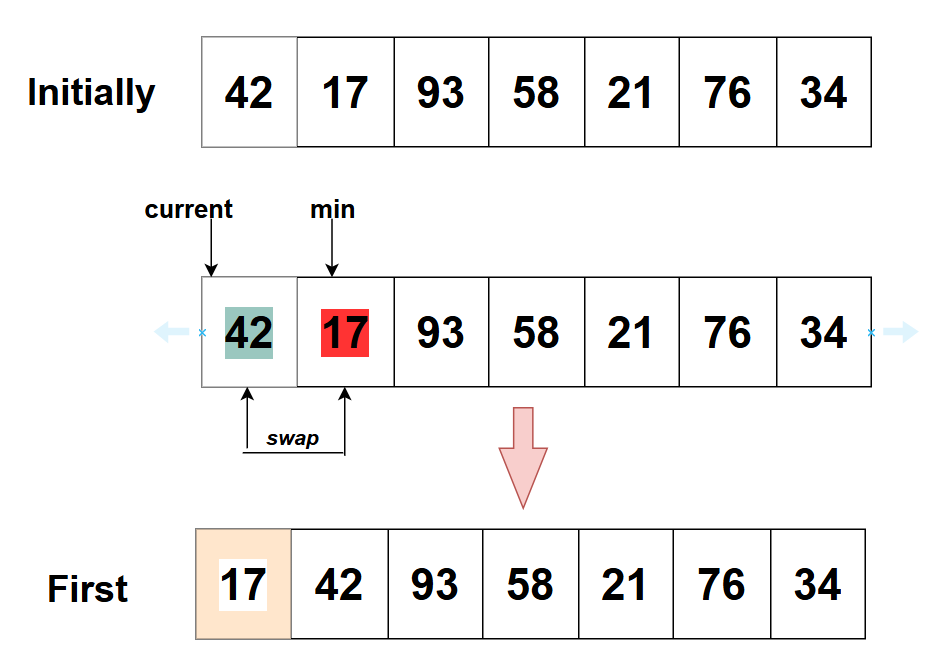
\includegraphics[width=0.7\textwidth]{img/selection sort/1.png}
    
\end{figure}

\begin{itemize}
\item Bắt đầu với phần tử đầu tiên(vị trí \textbf{curr}), chạy từ \textbf{curr} đến cuối mảng tìm phần tử nhỏ nhất (vị trí \textbf{min}) rồi hoán đổi hai phần tử ở vị trí \textbf{curr} và \textbf{min}. 
\begin{figure}[H]
    \centering
    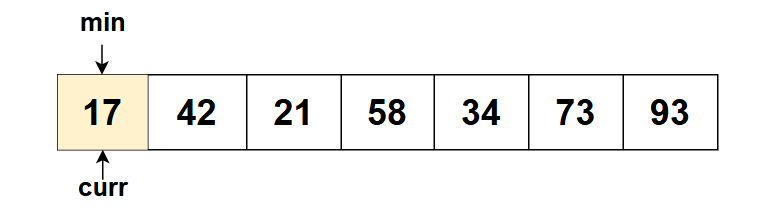
\includegraphics[width=0.7\textwidth]{img/selection sort/2.png}
    \caption{\textbf{curr} và \textbf{min} trùng nhau do 17 là phần tử nhỏ nhất}
\end{figure}

\begin{figure}[H]
    \centering
    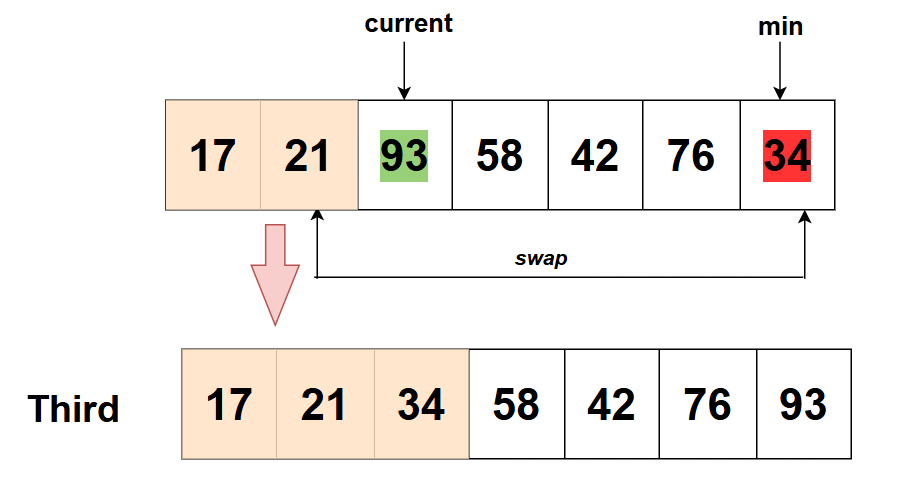
\includegraphics[width=0.7\textwidth]{img/selection sort/3.png}
    \caption{kết quả lần hoán vị đầu tiên.}
\end{figure}

\item Tiếp tục tăng \textbf{curr}, phần tử tiếp theo là vị trí \textbf{curr}, duyệt đến cuối mảng tìm phần tử nhỏ nhất (vị trí \textbf{min}) rồi hoán vị hai phần tử \textbf{curr} và \textbf{min}.

\begin{figure}[H]
    \centering
    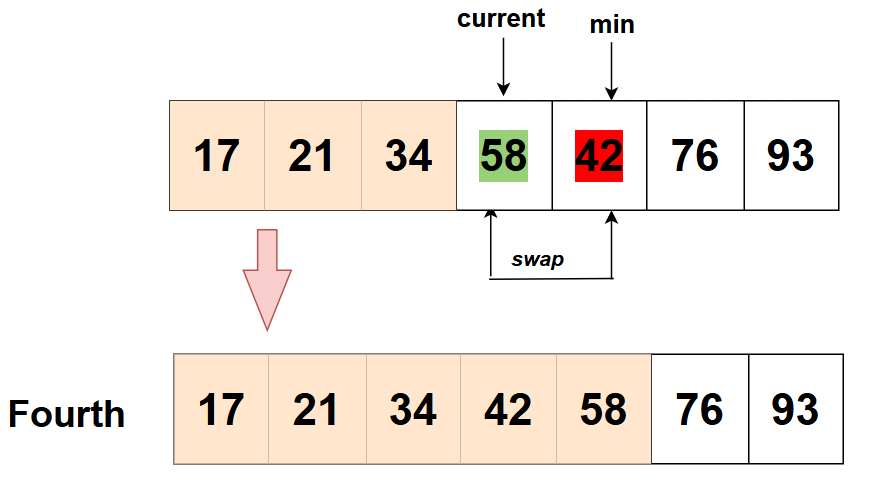
\includegraphics[width=0.7\textwidth]{img/selection sort/4.png}
    \caption{ta sẽ hoán đổi 42 và 21}
\end{figure}

\begin{figure}[H]
    \centering
    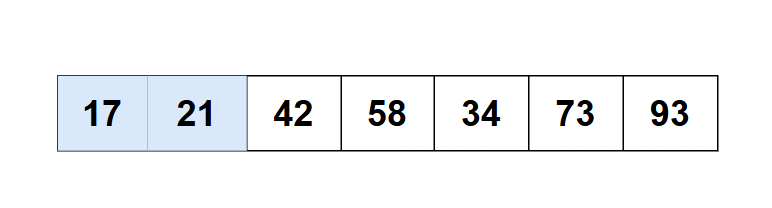
\includegraphics[width=0.7\textwidth]{img/selection sort/5.png}
    \caption{kết quả lần hoán vị thứ 2} 
\end{figure}

\item  Thực hiện tương tự cho đến khi mảng được sắp xếp.
\begin{figure}[H]
    \centering
    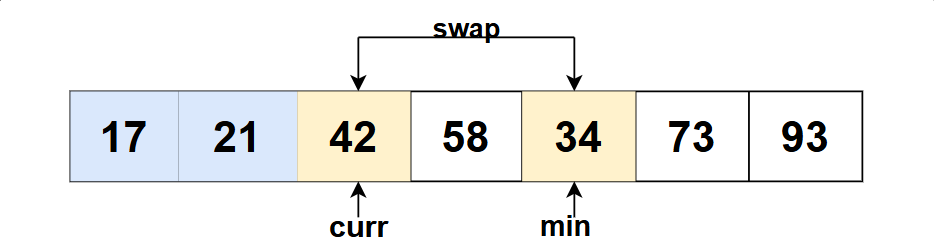
\includegraphics[width=0.7\textwidth]{img/selection sort/6.png} 
\end{figure}

\begin{figure}[H]
    \centering
    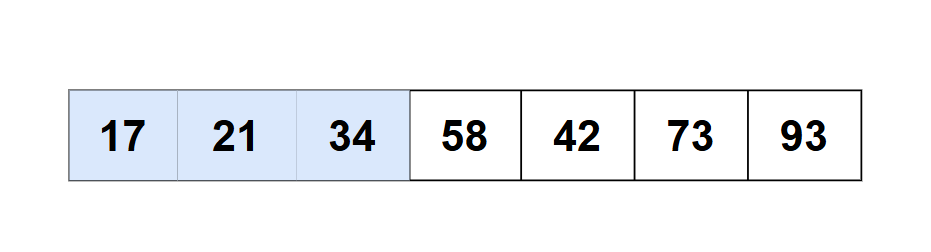
\includegraphics[width=0.7\textwidth]{img/selection sort/7.png} 
\end{figure}

\begin{figure}[H]
    \centering
    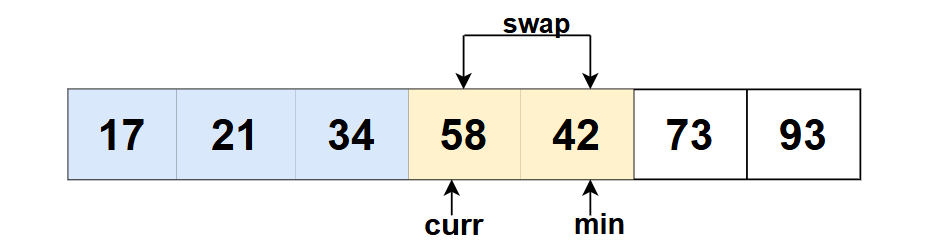
\includegraphics[width=0.7\textwidth]{img/selection sort/8.png} 
\end{figure}

\begin{figure}[H]
    \centering
    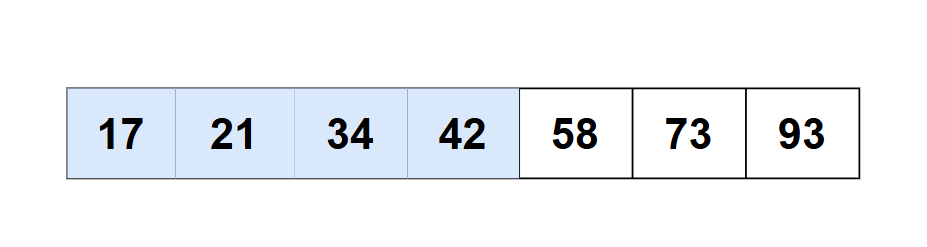
\includegraphics[width=0.7\textwidth]{img/selection sort/9.png} 
\end{figure}

\begin{figure}[H]
    \centering
    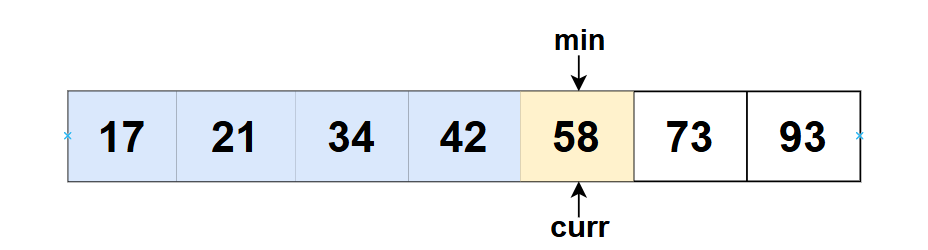
\includegraphics[width=0.7\textwidth]{img/selection sort/10.png} 
\end{figure}

\begin{figure}[H]
    \centering
    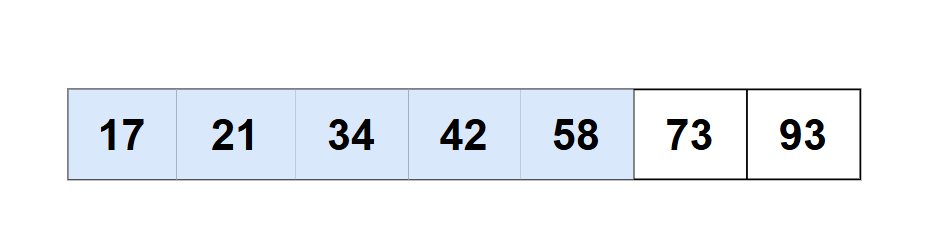
\includegraphics[width=0.7\textwidth]{img/selection sort/11.png} 
\end{figure}

\begin{figure}[H]
    \centering
    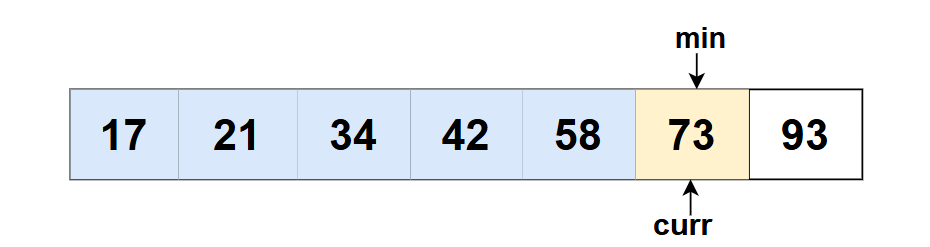
\includegraphics[width=0.7\textwidth]{img/selection sort/12.png} 
\end{figure}

\begin{figure}[H]
    \centering
    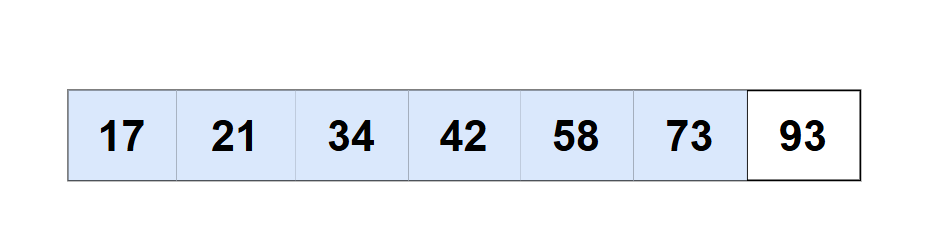
\includegraphics[width=0.7\textwidth]{img/selection sort/13.png} 
\end{figure}

\begin{figure}[H]
    \centering
    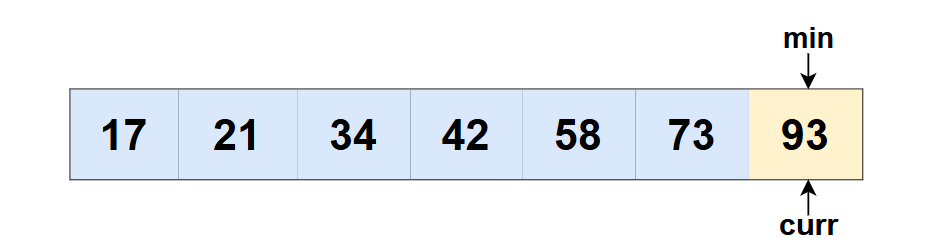
\includegraphics[width=0.7\textwidth]{img/selection sort/14.png} 
\end{figure}

\begin{figure}[H]
    \centering
    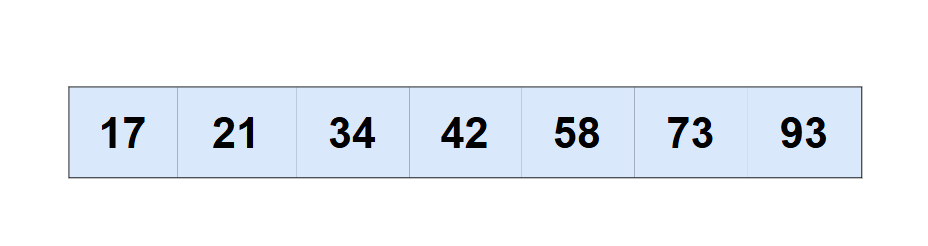
\includegraphics[width=0.7\textwidth]{img/selection sort/15.png} 
    \caption{Mảng đã được sắp xếp.}
\end{figure}


\end{itemize}

\subsubsection{{Độ phức tạp}}
\begin{itemize}
    \item[\textbf{--}] {Thời gian:}
    \begin{itemize}
        \item[$\bullet$] \textbf{Best Case:} \(\mathcal{O}(n^2)\), xảy ra ngay cả khi mảng đã được sắp xếp, vì thuật toán vẫn phải kiểm tra tất cả các phần tử để tìm giá trị nhỏ nhất trong mỗi lần lặp.
        \item[$\bullet$] \textbf{Average Case:} \(\mathcal{O}(n^2)\), trong trường hợp dữ liệu được phân bố ngẫu nhiên. Số lần so sánh và hoán đổi là cố định, không phụ thuộc vào cách dữ liệu được sắp xếp ban đầu.
        \item[$\bullet$] \textbf{Worst Case:} \(\mathcal{O}(n^2)\), xảy ra khi mảng ở trạng thái không sắp xếp. Thuật toán vẫn cần thực hiện \(n-1\) lần lặp, mỗi lần so sánh \(n-1\) phần tử còn lại.
    \end{itemize}
    \item[\textbf{--}] {Không gian:}
    \begin{itemize}
        \item[$\bullet$] Selection Sort là thuật toán \textbf{không yêu cầu bộ nhớ bổ sung} (\textbf{in-place}), vì nó chỉ sử dụng một biến phụ để lưu trữ giá trị tạm thời trong quá trình hoán đổi.
        \item[$\bullet$] Độ phức tạp bộ nhớ là:
        \[
        \mathcal{O}(1)
        \]
    \end{itemize}
    \item[\textbf{--}] {Tính ổn định:}
    \begin{itemize}
        \item[$\bullet$] Selection Sort là một thuật toán \textbf{không ổn định}. Khi hai phần tử có giá trị bằng nhau, vị trí tương đối của chúng có thể thay đổi sau quá trình hoán đổi.
    \end{itemize}
\end{itemize}
\newpage

\subsection{Insertion Sort}
\subsubsection{Ý tưởng}
Insertion sort là một thuật toán sắp xếp đơn giản hoạt động bằng cách lặp lại việc chèn từng phần tử của một danh sách chưa được sắp xếp vào đúng vị trí của nó trong một phần đã được sắp xếp của danh sách. Nó giống như việc sắp xếp các lá bài trong tay bạn. Bạn chia các lá bài thành hai nhóm: các lá bài đã được sắp xếp và các lá bài chưa được sắp xếp. Sau đó, bạn chọn một lá bài từ nhóm chưa được sắp xếp và đặt nó vào đúng vị trí trong nhóm đã được sắp xếp.
\subsubsection{Mã giả}

\begin{algorithm}[H]
\caption{Insertion sort}
\begin{algorithmic}[1]
\Procedure{BubbleSort}{$arr, n$}
    \State \textbf{Input:} Mảng $arr$ gồm $n$ phần tử
    \State \textbf{Output:} Mảng $arr$ được sắp xếp
    
    \For {$i \gets 0 $ \textbf{to} $n$}
        \For {$j \gets 0$ \textbf{to} $n - i - 1$} 
            \If{$arr[j] > arr[j+1]$}
                \State \textbf{swap} $arr[j]$ \textbf{and} $arr[j+1]$
            \EndIf
        \EndFor
    \EndFor
\EndProcedure
\end{algorithmic}
\end{algorithm}

\subsubsection{Ví dụ}

\begin{figure}[H]
    \centering
    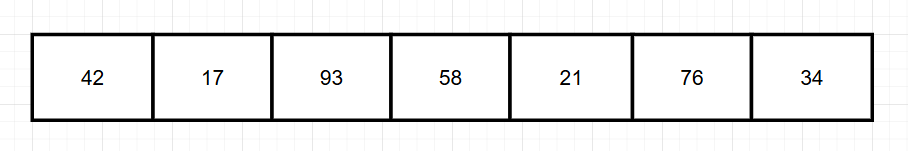
\includegraphics[width=1\linewidth]{img/bubble_sort/1.png}
    
    \vspace{0.5cm}
    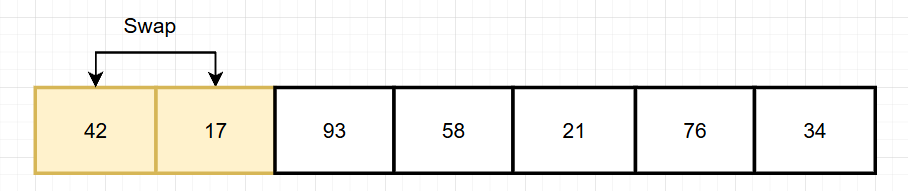
\includegraphics[width=1\linewidth]{img/bubble_sort/2.png}
    \vspace{0.5cm}
    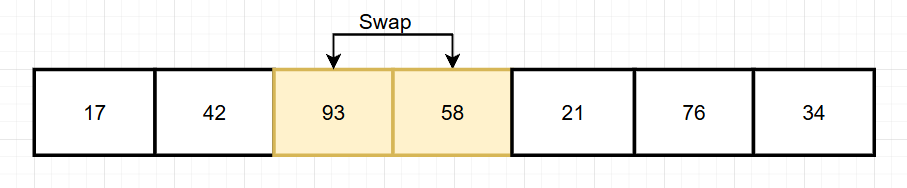
\includegraphics[width=1\linewidth]{img/bubble_sort/3.png}
    \vspace{0.5cm}
    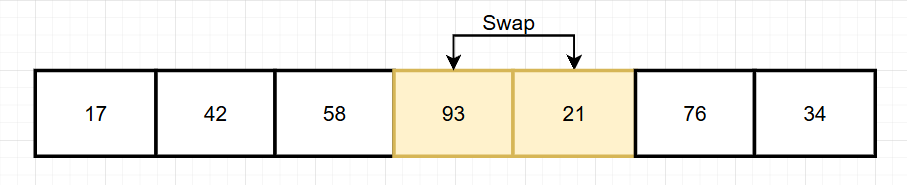
\includegraphics[width=1\linewidth]{img/bubble_sort/4.png}
    \vspace{0.5cm}
    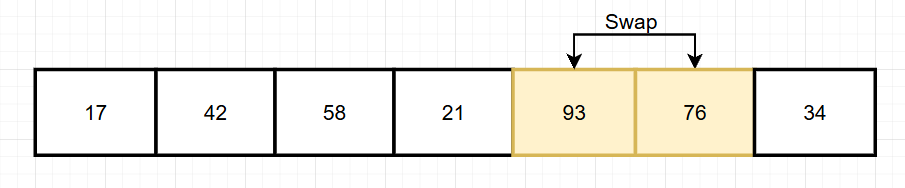
\includegraphics[width=1\linewidth]{img/bubble_sort/5.png}
    \caption{Các bước chạy - 1}
    \label{fig:part1}
\end{figure}

\begin{figure}[H]
    \centering
    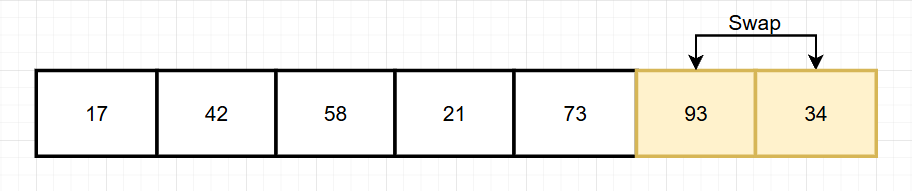
\includegraphics[width=1\linewidth]{img/bubble_sort/6.png}
    
    \vspace{0.5cm}
    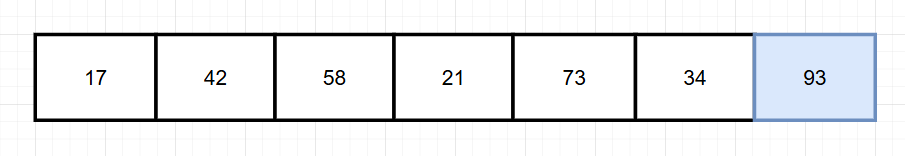
\includegraphics[width=1\linewidth]{img/bubble_sort/7.png}
    \vspace{0.5cm}
    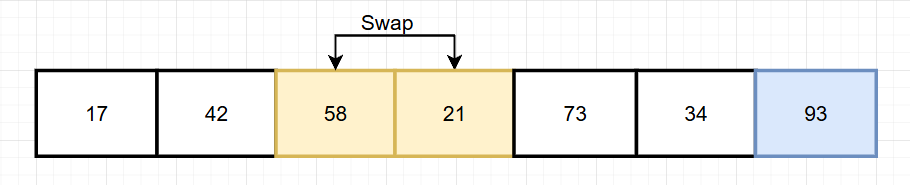
\includegraphics[width=1\linewidth]{img/bubble_sort/8.png}
    \vspace{0.5cm}
    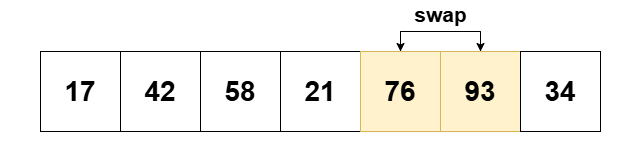
\includegraphics[width=1\linewidth]{img/bubble_sort/9.png}
    \vspace{0.5cm}
    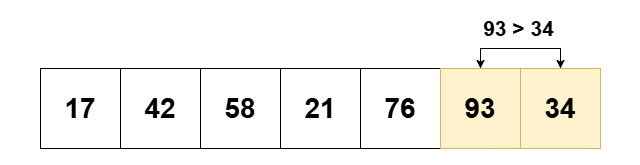
\includegraphics[width=1\linewidth]{img/bubble_sort/10.png}
    \caption{Các bước chạy - 2}
    \label{fig:part2}
\end{figure}

\begin{figure}[H]
    \centering
    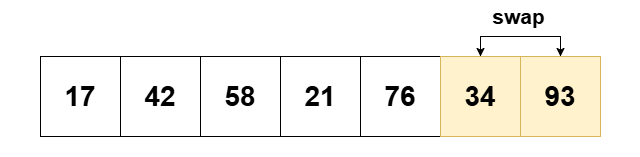
\includegraphics[width=1\linewidth]{img/bubble_sort/11.png}
    
    \vspace{0.5cm}
    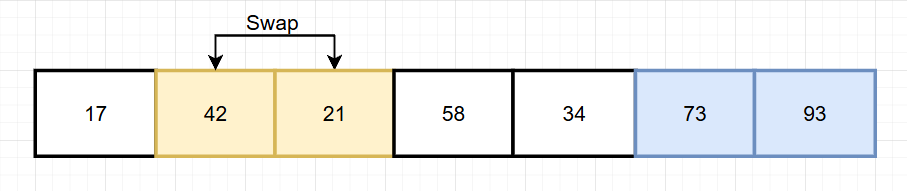
\includegraphics[width=1\linewidth]{img/bubble_sort/12.png}
    \vspace{0.5cm}
    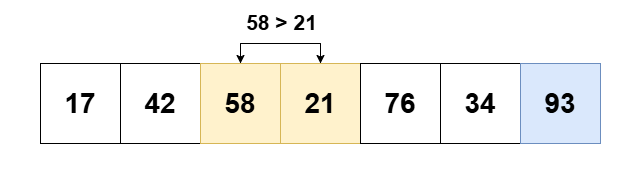
\includegraphics[width=1\linewidth]{img/bubble_sort/13.png}
    \vspace{0.5cm}
    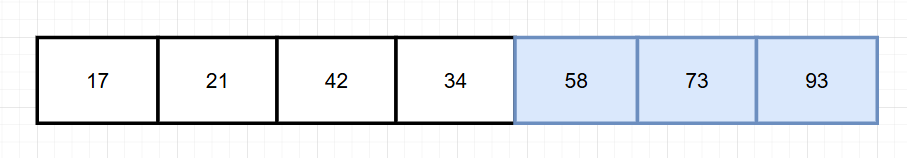
\includegraphics[width=1\linewidth]{img/bubble_sort/14.png}
    \vspace{0.5cm}
    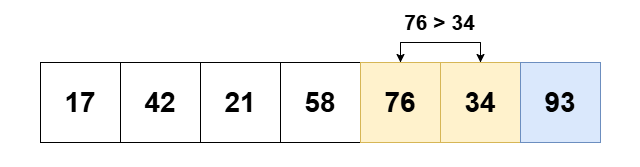
\includegraphics[width=1\linewidth]{img/bubble_sort/15.png}
    \caption{Các bước chạy - 3}
    \label{fig:part3}
\end{figure}

\begin{figure}[H]
    \centering
    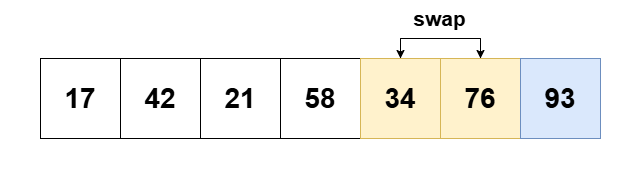
\includegraphics[width=1\linewidth]{img/bubble_sort/16.png}
    
    \vspace{0.5cm}
    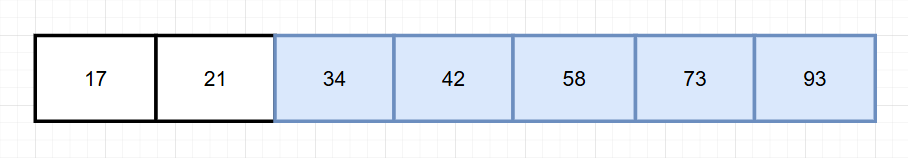
\includegraphics[width=1\linewidth]{img/bubble_sort/17.png}
    \vspace{0.5cm}
    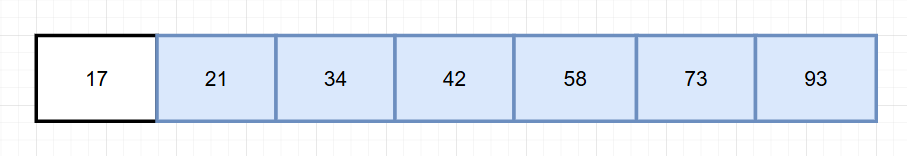
\includegraphics[width=1\linewidth]{img/bubble_sort/18.png}
    \vspace{0.5cm}
    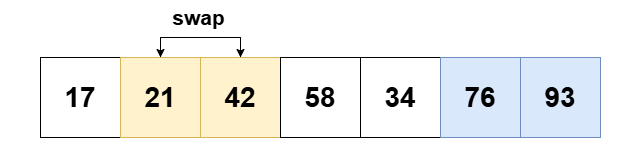
\includegraphics[width=1\linewidth]{img/bubble_sort/19.png}
    \caption{Các bước chạy - 4}
    \label{fig:part4}
\end{figure}


\subsubsection{Độ phức tạp}
\newpage
\subsection{Bubble Sort}
\subsubsection{Ý tưởng}
Bubble Sort là thuật toán sắp xếp so sánh liên tiếp các cặp phần tử liền kề trong mảng và hoán đổi nếu chúng không theo đúng thứ tự. Quá trình này được lặp lại cho đến khi mảng được sắp xếp. Với mỗi lần lặp, các phần tử sẽ được đưa về đúng vị trí của nó, giống như các bong bóng nổi lên từ dưới đáy nước. 
\subsubsection{Mã giả}

\begin{algorithm}[H]
\caption{BubbleSort}
\begin{algorithmic}[1]
\Procedure{BubbleSort}{$arr, n$}
    \State \textbf{Input:} Mảng $arr$ gồm $n$ phần tử
    \State \textbf{Output:} Mảng $arr$ được sắp xếp
    
    \For {$i \gets 0 $ \textbf{to} $n$}
        \For {$j \gets 0$ \textbf{to} $n - i - 1$} 
            \If{$arr[j] > arr[j+1]$}
                \State \textbf{swap} $arr[j]$ \textbf{and} $arr[j+1]$
            \EndIf
        \EndFor
    \EndFor
\EndProcedure
\end{algorithmic}
\end{algorithm}

\subsubsection{Ví dụ}

Dưới đây là các bước chạy tay của thuật toán \textit{Bubble Sort} với mảng $[42, 17, 93, 58, 21, 76, 34]$:
\begin{figure}[H]
    \centering
    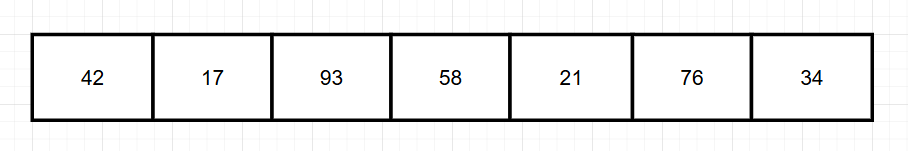
\includegraphics[width=0.75\linewidth]{img/bubble_sort/1.png}
\end{figure}
\newpage
\begin{enumerate}
    \item Lần lặp thứ nhất
    \begin{figure}[H]
        \centering
        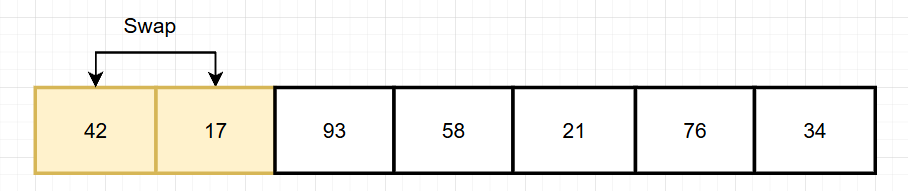
\includegraphics[width=0.75\linewidth]{img/bubble_sort/2.png}
        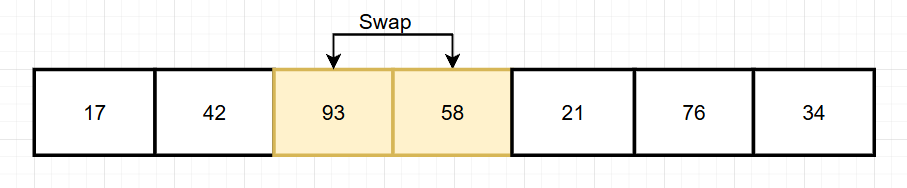
\includegraphics[width=0.75\linewidth]{img/bubble_sort/3.png}
        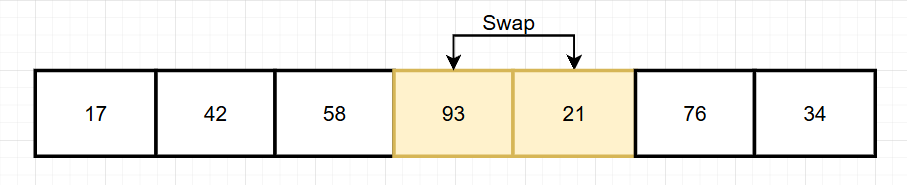
\includegraphics[width=0.75\linewidth]{img/bubble_sort/4.png}
        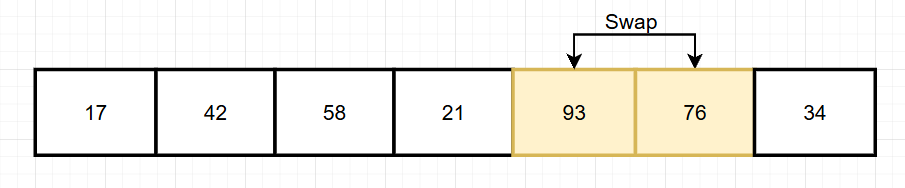
\includegraphics[width=0.75\linewidth]{img/bubble_sort/5.png}
        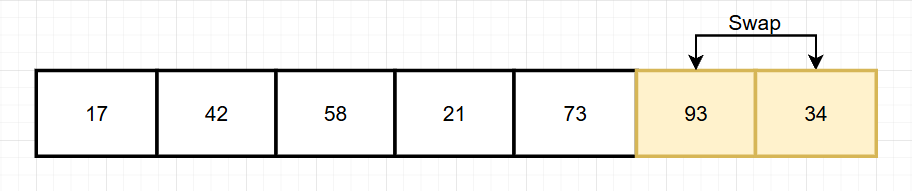
\includegraphics[width=0.75\linewidth]{img/bubble_sort/6.png}
        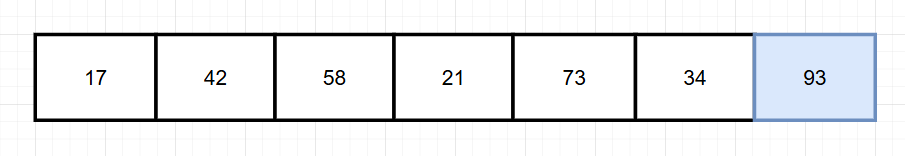
\includegraphics[width=0.75\linewidth]{img/bubble_sort/7.png}
    \end{figure}

    \begin{figure}[H]
        \centering
        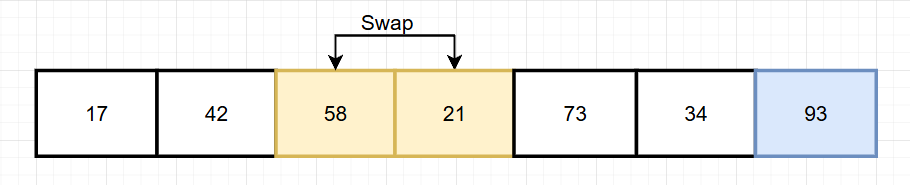
\includegraphics[width=0.75\linewidth]{img/bubble_sort/8.png}
        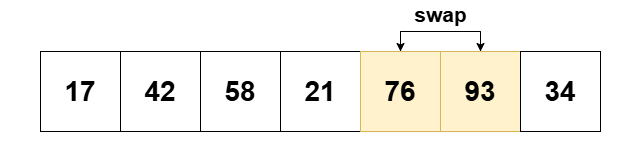
\includegraphics[width=0.75\linewidth]{img/bubble_sort/9.png}
        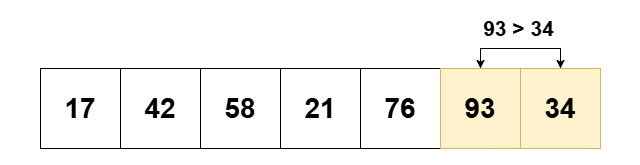
\includegraphics[width=0.75\linewidth]{img/bubble_sort/10.png}
        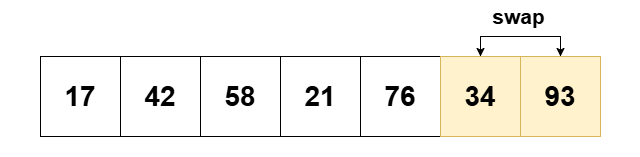
\includegraphics[width=0.75\linewidth]{img/bubble_sort/11.png}
        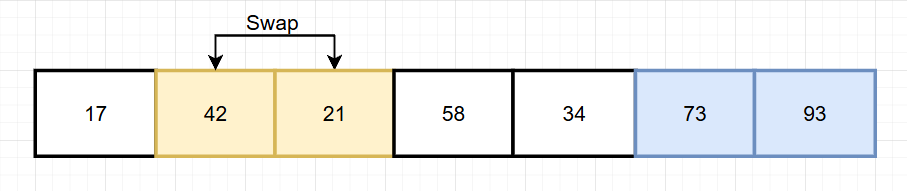
\includegraphics[width=0.75\linewidth]{img/bubble_sort/12.png}
    \end{figure}

    \item Lần lặp thứ hai
    \begin{figure}[H]
        \centering
        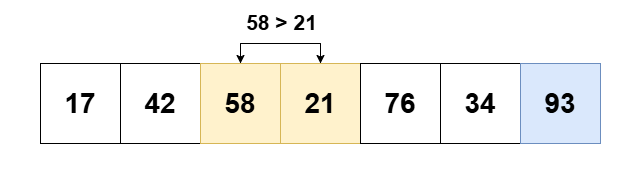
\includegraphics[width=0.75\linewidth]{img/bubble_sort/13.png}
       
    \end{figure}

    \begin{figure}[H]
        \centering
        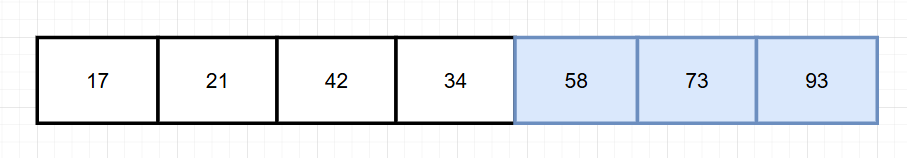
\includegraphics[width=0.75\linewidth]{img/bubble_sort/14.png} 
        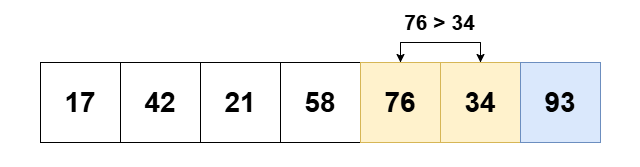
\includegraphics[width=0.75\linewidth]{img/bubble_sort/15.png}
        \includegraphics[width=0.75\linewidth]{img/bubble_sort/16.png}
        \includegraphics[width=0.75\linewidth]{img/bubble_sort/17.png}        
    \end{figure}

    \item Lần lặp thứ ba
    \begin{figure}[H]
        \centering
        \includegraphics[width=0.75\linewidth]{img/bubble_sort/18.png}
        \includegraphics[width=0.75\linewidth]{img/bubble_sort/19.png}
    \end{figure}

    \begin{figure}[H]
        \centering
        \includegraphics[width=0.75\linewidth]{img/bubble_sort/20.png}
        \includegraphics[width=0.75\linewidth]{img/bubble_sort/21.png}
        \includegraphics[width=0.75\linewidth]{img/bubble_sort/22.png}
    \end{figure}

    \item Lần lặp thứ tư
    \begin{figure}[H]
        \centering
        \includegraphics[width=0.75\linewidth]{img/bubble_sort/23.png}
        \includegraphics[width=0.75\linewidth]{img/bubble_sort/24.png}
        \includegraphics[width=0.75\linewidth]{img/bubble_sort/25.png}
    \end{figure}
    \newpage
    \item Lần lặp thứ năm
    \begin{figure}[H]
        \centering
        \includegraphics[width=0.75\linewidth]{img/bubble_sort/26.png}
    \end{figure}

    \item Lần lặp thứ sáu
    \begin{figure}[H]
        \centering
        \includegraphics[width=0.75\linewidth]{img/bubble_sort/27.png}
    \end{figure}

    \item Lần lặp thứ bảy
    \begin{figure}[H]
        \centering
        \includegraphics[width=0.75\linewidth]{img/bubble_sort/28.png}
    \end{figure}

    \item Cuối cùng ta thu được mảng được sắp xếp
    \begin{figure}[H]
        \centering
        \includegraphics[width=0.75\linewidth]{img/bubble_sort/28.png}
    \end{figure}
\end{enumerate}
\newpage
\subsubsection{Độ phức tạp}

\begin{itemize}
    \item[\textbf{--}]Độ phức tạp về thời gian:
        \begin{itemize}
            \item[\textbullet]\textbf{Best case}: $\mathcal{O}(n^2)$
            \item[\textbullet]\textbf{Average case}:  $\mathcal{O}(n^2)$
            \item[\textbullet]\textbf{Worst case}:  $\mathcal{O}(n^2)$
        \end{itemize}
    \item[\textbf{--}]Độ phức tạp về không gian:  $\mathcal{O}(1)$, vì không cần thêm bộ nhớ phụ nào trong quá trình sắp xếp.
    \item[\textbf{--}]Tính ổn định: \textit{Bubble sort} là thuật toán ổn định nghĩa là nó không thay đổi vị trí của các phần tử bằng nhau trong quá trình sắp xếp.
\newpage

\subsection{Shaker Sort}
\subsubsection{Ý tưởng}

Shaker Sort là một biến thể của Bubble Sort, nơi mà mảng được duyệt từ trái sang phải và từ phải sang trái xen kẽ. Thuật toán này giúp giảm số lần so sánh giữa các phần tử trong mảng bằng cách sắp xếp các phần tử lớn nhất và nhỏ nhất về hai phía của mảng. \cite{black2009}

\subsubsection{Mã giả}

\begin{algorithm}[H]
\caption{Shaker Sort}
\begin{algorithmic}[1]
\Function{ShakerSort}{$arr, n$}
    \State $left \gets 0$
    \State $right \gets n - 1$
    \While{$left < right$}
        \For{$i \gets left$ \textbf{to} $right - 1$}
            \If{$arr[i] > arr[i + 1]$}
                \State \Call{Swap}{$arr[i], arr[i + 1]$}
            \EndIf
        \EndFor
        \State $right \gets right - 1$
        \For{$i \gets right$ \textbf{downto} $left + 1$}
            \If{$arr[i] < arr[i - 1]$}
                \State \Call{Swap}{$arr[i], arr[i - 1]$}
            \EndIf
        \EndFor
        \State $left \gets left + 1$
    \EndWhile
    \State \textbf{return} $arr$
\EndFunction
\end{algorithmic}
\end{algorithm}

\subsubsection{Ví dụ}

\begin{enumerate}
    \item \textbf{Bước 1}: Khai báo 2 biến tạm $left$ và $right$ lần lượt là vị trí bắt đầu và kết thúc của mảng.
    \item \textbf{Bước 2}: Duyệt mảng từ trái sang phải và từ phải sang trái xen kẽ:
        \begin{itemize}
            \item Nếu phần tử hiện tại lớn hơn phần tử kế tiếp, ta đổi chỗ 2 phần tử này.
            \item Sau mỗi lần duyệt, ta cập nhật lại vị trí của $left$ và $right$ bằng cách tăng hoặc giảm giá trị của chúng đi $1$.
        \end{itemize}
    \item \textbf{Bước 3}: Lặp lại bước 2 cho đến khi $left \geq right$.
\end{enumerate}

\begin{figure}[H]
    \centering
    \includegraphics[width=0.6\linewidth]{img/shaker_sort/1.png}
    \caption{Quá trình thực hiện Shaker Sort}
\end{figure}

\subsubsection{Độ phức tạp}

\begin{itemize}
    \item[\textbf{--}] Độ phức tạp thời gian: 
    \begin{itemize}
        \item[$\bullet$] \textbf{Best case}: $\mathcal{O}(n^2)$
        \item[$\bullet$] \textbf{Average case}: $\mathcal{O}(n^2)$
        \item[$\bullet$] \textbf{Worst case}: $\mathcal{O}(n^2)$
    \end{itemize}
    \item[\textbf{--}] Độ phức tạp không gian:
    \begin{itemize}
        \item[$\bullet$] \textit{Shaker sort} không sử dụng thêm bộ nhớ phụ ngoài 2 biến tạm $left$ và $right$.
        \item[$\bullet$] Độ phức tạp bộ nhớ là:
        \[
        \mathcal{O}(1)
        \]
    \end{itemize}
    \item[\textbf{--}] Tính ổn định: \textit{Shaker Sort} là một thuật toán ổn định. Điều này có nghĩa là nếu có hai phần tử bằng nhau, thì chúng sẽ không bị đảo lộn thứ tự sau khi sắp xếp.
\end{itemize}

\newpage


\subsection{Shell Sort}
\subsubsection{Ý tưởng}
\textbf{Shell Sort} là một cải tiến của thuật toán \textbf{Insertion Sort}. Ý tưởng chính là sắp xếp các phần tử nằm xa nhau trước, sau đó giảm dần khoảng cách giữa các phần tử so sánh, và cuối cùng thực hiện một lần \textbf{Insertion Sort} với các khoảng cách bằng 1. Điều này giúp giảm số lần hoán đổi và so sánh khi so sánh các phần tử gần nhau ở bước cuối.

\subsubsection{Mã giả}
\begin{algorithm}[H]
\caption{ShellSort}
\begin{algorithmic}[1]
\Procedure{\textbf{ShellSort}}{$arr, n$}
    \State \textbf{Input:} Mảng $arr$ gồm $n$ phần tử
    \State \textbf{Output:} Mảng $arr$ được sắp xếp
    \State $gap \gets n/2$
    \While {$gap > 0$}
        \For {$i \gets gap$ \textbf{to} $n - 1$} 
            \State $temp \gets arr[i]$
            \State $j \gets i$
            \While{$j \geq gap$ \textbf{and} $arr[j - gap] > temp$}
                \State $arr[j] \gets arr[j - gap]$
                \State $j \gets j - gap$
            \EndWhile
            \State $arr[j] \gets temp$
        \EndFor
        \State $gap \gets gap / 2$
    \EndWhile
\EndProcedure
\end{algorithmic}
\end{algorithm}
\subsubsection{Ví dụ}
Dưới đây là các bước chạy tay của thuật toán \textbf{Shell Sort}:
\begin{figure}[H]
    \centering
    \includegraphics[width=1\linewidth]{img/shell_sort/1.png}
    \vspace{0.15cm}
    \includegraphics[width=1\linewidth]{img/shell_sort/2.png}
    \vspace{0.15cm}
    \includegraphics[width=1\linewidth]{img/shell_sort/3.png}
    \vspace{0.15cm}
    \includegraphics[width=1\linewidth]{img/shell_sort/4.png}
    \caption{Các bước chạy - 1}
    \label{fig:part1}
\end{figure}

\begin{figure}[H]
    \centering
    \includegraphics[width=1\linewidth]{img/shell_sort/5.png}
    \vspace{0.5cm}
    \includegraphics[width=1\linewidth]{img/shell_sort/6.png}
    \vspace{0.15cm}
    \includegraphics[width=1\linewidth]{img/shell_sort/7.png}
    \vspace{0.15cm}
    \includegraphics[width=1\linewidth]{img/shell_sort/8.png}
    \caption{Các bước chạy - 2}
    \label{fig:part2}
\end{figure}

\begin{figure}[H]
    \centering
    \includegraphics[width=1\linewidth]{img/shell_sort/09.png}
    \vspace{0.15cm}
    \includegraphics[width=1\linewidth]{img/shell_sort/10.png}
    \vspace{0.15cm}
    \includegraphics[width=1\linewidth]{img/shell_sort/11.png}
    \vspace{0.15cm}
    \includegraphics[width=1\linewidth]{img/shell_sort/12.png}
    \caption{Các bước chạy - 3}
    \label{fig:part3}
\end{figure}

\begin{figure}[H]
    \centering
    \includegraphics[width=1\linewidth]{img/shell_sort/13.png}
    \vspace{0.15cm}
    \includegraphics[width=1\linewidth]{img/shell_sort/14.png}
    \vspace{0.15cm}
    \includegraphics[width=1\linewidth]{img/shell_sort/15.png}
    \vspace{0.15cm}
    \includegraphics[width=1\linewidth]{img/shell_sort/16.png}
    \caption{Các bước chạy - 4}
    \label{fig:part4}
\end{figure}

\begin{figure}[H]
    \centering
    \includegraphics[width=1\linewidth]{img/shell_sort/17.png}
    \vspace{0.15cm}
    \includegraphics[width=1\linewidth]{img/shell_sort/18.png}
    \vspace{0.15cm}
    \includegraphics[width=1\linewidth]{img/shell_sort/19.png}
    \vspace{0.15cm}
    \includegraphics[width=1\linewidth]{img/shell_sort/20.png}
    \caption{Các bước chạy - 5}
    \label{fig:part5}
\end{figure}

\begin{figure}[H]
    \centering
    \includegraphics[width=1\linewidth]{img/shell_sort/21.png}
    \vspace{0.15mm}
    \includegraphics[width=1\linewidth]{img/shell_sort/22.png}
    \vspace{0.15mm}
    \includegraphics[width=1\linewidth]{img/shell_sort/23.png}
    \vspace{0.15mm}
    \includegraphics[width=1\linewidth]{img/shell_sort/24.png}
    \vspace{0.15mm}
    \includegraphics[width=1\linewidth]{img/shell_sort/25.png}
    \caption{Các bước chạy - 6}
    \label{fig:part6}
\end{figure}

\subsubsection{Độ phức tạp}
\begin{itemize}
    \item[\textbf{--}] \textbf{Độ phức tạp về thời gian:}
    \begin{itemize}
        \item[$\bullet$] \textbf{Best Case:} $\mathcal{O}(n \cdot \log n)$, phụ thuộc vào cách chọn chuỗi khoảng cách (gap sequence). Khi mảng gần như đã được sắp xếp, số phép hoán đổi và so sánh giảm đáng kể.
        \item[$\bullet$] \textbf{Average Case:} $\mathcal{O}(n^{3/2})$, đối với chuỗi khoảng cách phổ biến như Knuth hoặc Hibbard. Đây là độ phức tạp trung bình được quan sát trong thực tế và lý thuyết.
        \item[$\bullet$] \textbf{Worst Case:} $\mathcal{O}(n^2)$, xảy ra khi mảng có cấu trúc dữ liệu bất lợi hoặc chuỗi khoảng cách không được tối ưu hóa.
    \end{itemize}
    \item[\textbf{--}] \textbf{Độ phức tạp về không gian:} $\mathcal{O}(1)$, do thuật toán thực hiện in-place, không yêu cầu bộ nhớ phụ trợ.
    \item[\textbf{--}] \textbf{Tính ổn định:} Thuật toán không ổn định, vì trong quá trình di chuyển các phần tử qua khoảng cách lớn, thứ tự ban đầu của các phần tử có giá trị bằng nhau có thể bị thay đổi.
\end{itemize}

\newpage

\subsection{Heap Sort}
\subsubsection{Ý tưởng}
\textbf{Heap Sort} là thuật toán sắp xếp dựa trên cấu trúc dữ liệu \textbf{Binary Heap}, trong đó phần tử lớn nhất (hoặc nhỏ nhất) được đưa về gốc của \textit{heap} (\textit{max heap} hoặc \textit{min heap}). Sau đó, phần tử này được hoán đổi với phần tử cuối mảng và loại bỏ khỏi \textit{heap}. Quá trình xây dựng lại \textit{heap} và hoán đổi được lặp lại cho đến khi mảng được sắp xếp.

\subsubsection{Mã giả}
\begin{algorithm}[H]
\caption{Heap Sort}
\begin{algorithmic}[1]
\Procedure{HeapSort}{$arr, n$}
    \State \textbf{Input:} Mảng $arr$ gồm $n$ phần tử
    \State \textbf{Output:} Mảng $arr$ được sắp xếp
    
    \For {$i \gets n /2 -1 $ \textbf{downto} $0$}
        \State \Call {Heapify}{$arr, n, i$}
    \EndFor
    
    \For {$i \gets n - 1$ \textbf{downto} $0$}
        \State \textbf{swap} $arr[0]$ \textbf{and} $arr[i]$
        \State \Call {heapify}{$arr, i, 0$}
    \EndFor
\EndProcedure
\Procedure{Heapify}{$arr, n, i$}
    \State $largest \gets i$
    \State $left \gets 2\times i + 1$
    \State $right \gets 2\times i + 2$
    \If {$left < n$ \textbf{and} $arr[largest] < arr[left]$}
        \State $largest \gets left$
    \EndIf
    \If {$right < n$ \textbf{and} $arr[largest] < arr[right]$}
        \State $largest \gets right$
    \EndIf
    \If {$largest \ne i$}
        \State \textbf{swap} $arr[i]$ \textbf{and} $arr[largest]$
        \State \Call {heapify}{$arr, n, largest$}
    \EndIf
\EndProcedure
\end{algorithmic}
\end{algorithm}

\subsubsection{Ví dụ}
Dưới đây là các bước chạy tay của thuật toán \textbf{Heap Sort}:

\begin{itemize}
    \item [\textbf{--}] Đầu tiên chúng ta sẽ xây dựng \textbf{max heap}:
\end{itemize}

\begin{figure}[H]
    \centering
    \includegraphics[width=0.5\linewidth]{img/heap_sort/1.png}
    \vspace{0.01cm}

    \includegraphics[width=0.1\linewidth]{img/heap_sort/arrow.png}
    \vspace{0.01cm}

    \includegraphics[width=0.5\linewidth]{img/heap_sort/2.png}
    \vspace{0.01cm}

    \includegraphics[width=0.1\linewidth]{img/heap_sort/arrow.png}
    \vspace{0.01cm}

    \includegraphics[width=0.5\linewidth]{img/heap_sort/3.png}

    \caption{Các bước xây dựng \textit{max heap} - 1}
\end{figure}

\begin{figure}[H]
    \centering
    \includegraphics[width=0.1\linewidth]{img/heap_sort/arrow.png}
    \vspace{0.01cm}

    \includegraphics[width=0.5\linewidth]{img/heap_sort/4.png}
    \vspace{0.01cm}

    \includegraphics[width=0.1\linewidth]{img/heap_sort/arrow.png}
    \vspace{0.01cm}
    
    \includegraphics[width=0.5\linewidth]{img/heap_sort/5.png}
    \vspace{0.01cm}

    \includegraphics[width=0.1\linewidth]{img/heap_sort/arrow.png}
    \vspace{0.01cm}

    \includegraphics[width=0.5\linewidth]{img/heap_sort/6.png}

    \caption{Các bước xây dựng \textit{max heap} - 2}
\end{figure}

\begin{figure}[H]
    \centering
    \includegraphics[width=0.1\linewidth]{img/heap_sort/arrow.png}
    \vspace{0.01cm}

    \includegraphics[width=0.5\linewidth]{img/heap_sort/7.png}

    \caption{Xây dựng thành công \textit{max heap} - 3}
\end{figure}

\begin{itemize}
    \item [\textbf{--}] Từ \textbf{max heap} vừa xây dựng ta sẽ hoán đổi phần tử ở nút gốc với phần tử cuối cùng, rồi giảm kích thước của \textbf{Heap} đi 1, sau đó thực hiện lại thao tác \textbf{Heapify} (xây dựng \textit{max heap}):
\end{itemize}

\begin{figure}[H]
    \centering
    \includegraphics[width=0.5\linewidth]{img/heap_sort/8.png}
    \vspace{0.01cm}

    \includegraphics[width=0.1\linewidth]{img/heap_sort/arrow.png}
    \vspace{0.01cm}

    \includegraphics[width=0.5\linewidth]{img/heap_sort/9.png}

    \caption{Các bước chạy thuật toán \textbf{Heap sort} - 4}
\end{figure}

\begin{figure}[H]
    \centering
    \includegraphics[width=0.1\linewidth]{img/heap_sort/arrow.png}
    \vspace{0.01cm}

    \includegraphics[width=0.5\linewidth]{img/heap_sort/10.png}
    \vspace{0.01cm}

    \includegraphics[width=0.1\linewidth]{img/heap_sort/arrow.png}
    \vspace{0.01cm}

    \includegraphics[width=0.5\linewidth]{img/heap_sort/11.png}
    \vspace{0.01cm}

    \includegraphics[width=0.1\linewidth]{img/heap_sort/arrow.png}
    \vspace{0.01cm}

    \includegraphics[width=0.5\linewidth]{img/heap_sort/12.png}

    \caption{Các bước chạy thuật toán \textbf{Heap sort} - 5}
\end{figure}

\begin{figure}[H]
    \centering
    \includegraphics[width=0.1\linewidth]{img/heap_sort/arrow.png}
    \vspace{0.01cm}

    \includegraphics[width=0.5\linewidth]{img/heap_sort/13.png}
    \vspace{0.01cm}

    \includegraphics[width=0.1\linewidth]{img/heap_sort/arrow.png}
    \vspace{0.01cm}

    \includegraphics[width=0.5\linewidth]{img/heap_sort/14.png}
    \vspace{0.01cm}

    \includegraphics[width=0.1\linewidth]{img/heap_sort/arrow.png}
    \vspace{0.01cm}

    \includegraphics[width=0.5\linewidth]{img/heap_sort/15.png}

    \caption{Các bước chạy thuật toán \textbf{Heap sort} - 6}
\end{figure}

\begin{figure}[H]
    \centering
    \includegraphics[width=0.1\linewidth]{img/heap_sort/arrow.png}
    \vspace{0.01cm}

    \includegraphics[width=0.5\linewidth]{img/heap_sort/16.png}
    \vspace{0.01cm}

    \includegraphics[width=0.1\linewidth]{img/heap_sort/arrow.png}
    \vspace{0.01cm}

    \includegraphics[width=0.5\linewidth]{img/heap_sort/17.png}
    \vspace{0.01cm}

    \includegraphics[width=0.1\linewidth]{img/heap_sort/arrow.png}
    \vspace{0.01cm}

    \includegraphics[width=0.5\linewidth]{img/heap_sort/18.png}

    \caption{Các bước chạy thuật toán \textbf{Heap sort} - 7}
\end{figure}

\begin{figure}[H]
    \centering
    \includegraphics[width=0.1\linewidth]{img/heap_sort/arrow.png}
    \vspace{0.01cm}

    \includegraphics[width=0.5\linewidth]{img/heap_sort/19.png}
    \vspace{0.01cm}

    \includegraphics[width=0.1\linewidth]{img/heap_sort/arrow.png}
    \vspace{0.01cm}

    \includegraphics[width=0.5\linewidth]{img/heap_sort/20.png}
    \vspace{0.01cm}

    \includegraphics[width=0.1\linewidth]{img/heap_sort/arrow.png}
    \vspace{0.01cm}

    \includegraphics[width=0.5\linewidth]{img/heap_sort/21.png}

    \caption{Các bước chạy thuật toán \textbf{Heap sort} - 8}
\end{figure}

\begin{figure}[H]
    \centering
    \includegraphics[width=0.1\linewidth]{img/heap_sort/arrow.png}
    \vspace{0.5cm}

    \includegraphics[width=0.5\linewidth]{img/heap_sort/22.png}
    \vspace{0.5cm}

    \includegraphics[width=0.1\linewidth]{img/heap_sort/arrow.png}
    \vspace{0.5cm}

    \includegraphics[width=0.5\linewidth]{img/heap_sort/23.png}

    \caption{Các bước chạy thuật toán \textbf{Heap sort} - 9}
\end{figure}
\subsubsection{Độ phức tạp}

\begin{itemize}
    \item [\textbf{--}] \textbf{Quá trình xây dựng Heap (Build Heap):}
    \begin{itemize}
        \item [$\bullet$] \textbf{Phân tích chi tiết:}
        \begin{itemize}
            \item [$\bullet$] Với mỗi nút ở cấp độ $i$, chi phí tái cấu trúc \textbf{Heap} (\textit{Heapify}) tỷ lệ với chiều cao của nút đó, $h_i$.
            \item [$\bullet$] Số lượng nút ở mỗi cấp đó $k$ của cây nhị phân là $2^k$, và chiều cao của cây là $\log n$.
            \item [$\bullet$] Tổng chi phí được tính bằng:
            \begin{center}
                $T_{\text{build}} = \sum_{k=0}^{\log n - 1} \frac{n}{2^{k+1}} \cdot k$
            \end{center}
            \item [$\bullet$] Sau khi triển khai bài toán và đơn giản hóa, ta có:
            \begin{center}
                $T_{\text{build}} = \mathcal{O}(n)$
            \end{center}
        \end{itemize}
    \end{itemize}
    \item [\textbf{--}] \textbf{Quá trình sắp xếp (Heap sort):}
    \begin{itemize}
        \item [$\bullet$] Sau khi xây dựng \textbf{Heap}, phần tử lớn nhất (gốc \textit{Heap}) được đưa về cuối mảng, và sau đó \textbf{Heapify} lại.
        \item [$\bullet$] \textbf{Chi phí tái cấu trúc Heap (\textit{Heapify}):}
        \begin{itemize}
            \item [$\bullet$] Tại mỗi bước, \textbf{Heapify} có độ phức tạp $\mathcal{O}(\log n)$.
            \item [$\bullet$] Tổng số bước là $n-1$ vì mỗi lần chỉ sắp xếp một phần tử.
            \item [$\bullet$] Tổng chi phí:
            \begin{center}
                $T_{\text{sort}} = \sum_{i=1}^{n-1} \mathcal{O}(\log i) = \mathcal{O}(n \cdot \log n)$
            \end{center}
        \end{itemize}
    \end{itemize}
    \item [\textbf{--}] \textbf{Độ phức tạp tổng quát:}
    \begin{itemize}
        \item [$\bullet$] Tổng độ phức tạp của \textbf{Heap sort} là tổng chi phí của việc xây dựng \textbf{Heap} và sắp xếp:
        \begin{center}
            $T_{\text{total}} = T_{\text{build}} + T_{\text{sort}} = \mathcal{O}(n) + \mathcal{O}(n \cdot \log n) = \mathcal{O}(n \cdot \log n)$
        \end{center}
    \end{itemize}
    \item [\textbf{--}] \textbf{Phân tích theo các trường hợp:}
    \begin{itemize}
        \item [$\bullet$] \textbf{Trường hợp tốt nhất}
        \begin{itemize}
            \item [$\bullet$] Trường hợp tốt nhất, \textbf{Heapify} vẫn phải thực hiện đầy đủ các bước, vì vậy không giảm độ phức tạp:
            \begin{center}
                $T_{\text{best}} = \mathcal{O}(n \cdot \log n)$
            \end{center}
        \end{itemize}
        \item [$\bullet$] \textbf{Trường hợp trung bình}
        \begin{itemize}
            \item [$\bullet$] Với các mảng ngẫu nhiên, sắp xếp, gần được sắp xếp, mảng giảm dần, trung bình mỗi lần \textbf{Heapify} vẫn có độ phức tạp $\mathcal{O}(\log n)$, lặp lại $n-1$ lần mà không phụ thuộc vào trạng thái ban đầu của mảng.
            \begin{center}
                $T_{\text{average}} = \mathcal{O}(n \cdot \log n)$
            \end{center}
        \end{itemize}
        \item [$\bullet$] \textbf{Trường hợp xấu nhất}
        \begin{itemize}
            \item [$\bullet$] Trường hợp xấu nhất cũng không khác biệt vì \textbf{Heapify} vẫn phải xử lý toàn bộ chiều của \textbf{Heap}.
            \begin{center}
                $T_{\text{worst}} = \mathcal{O}(n \cdot \log n)$
            \end{center}
        \end{itemize}
    \end{itemize}
    \item [\textbf{--}] \textbf{Không gian bộ nhớ:}
    \begin{itemize}
        \item [$\bullet$] \textbf{Heap sort} sử dụng \textbf{\textit{Heap in-place}} (trong cùng mảng), vì vậy độ phức tạp không gian là:
        \begin{center}
            $S = \mathcal{O}(1)$
        \end{center}
    \end{itemize}
    \item [\textbf{--}] \textbf{Độ ổn đinh:}
    \begin{itemize}
        \item [$\bullet$] \textbf{Heap sort không ổn định} vì quá trình hoán đổi giữa các phần tử có giá trị bằng nhau có thể làm thay đổi thứ tự của chúng.
    \end{itemize}
\end{itemize}

\newpage

\subsection{Merge Sort}
\subsubsection{Ý tưởng}
Merge Sort là một thuật toán sắp xếp chia để trị (divide-and-conquer). Thuật toán chia mảng ban đầu thành hai nửa, tiếp tục chia nhỏ từng nửa cho đến khi mỗi phần chỉ còn một phần tử. Sau đó, các phần nhỏ này được hợp nhất lại theo thứ tự sắp xếp để tạo thành mảng đã sắp xếp. \cite{drozdek2023}

\subsubsection{Mã giả}

\begin{algorithm}[H]
\caption{Merge Sort (Mảng bắt đầu từ 0)}
\begin{algorithmic}[1]
\Procedure{MergeSort}{$arr, left, right$}
    \State \textbf{Input:} Mảng $arr$ với chỉ số bắt đầu $left$ và kết thúc $right$
    \State \textbf{Output:} Mảng $arr$ được sắp xếp trong đoạn $[left, right]$
    
    \If{$left < right$}
        \State Tính chỉ số giữa $mid \gets \lfloor (left + right) / 2 \rfloor$
        
        \State \textbf{Chia nhỏ (Divide):}
        \State \Call{MergeSort}{$arr, left, mid$} \Comment{Đệ quy cho nửa trái}
        \State \Call{MergeSort}{$arr, mid+1, right$} \Comment{Đệ quy cho nửa phải}
        
        \State \textbf{Hợp nhất (Conquer):}
        \State \Call{Merge}{$arr, left, mid, right$} \Comment{Hợp nhất hai nửa đã sắp xếp}
    \EndIf
\EndProcedure

\Procedure{Merge}{$arr, left, mid, right$}
    \State \textbf{Input:} Mảng $arr$ với hai đoạn $[left, mid]$ và $[mid+1, right]$ đã được sắp xếp
    \State \textbf{Output:} Đoạn $[left, right]$ được sắp xếp
    
    \State Khởi tạo mảng tạm $L[0..(mid-left)]$ và $R[0..(right-mid-1)]$
    \For{$i \gets 0$ \textbf{to} $mid - left$}
        \State $L[i] \gets arr[left + i]$
    \EndFor
    \For{$j \gets 0$ \textbf{to} $right - mid - 1$}
        \State $R[j] \gets arr[mid + 1 + j]$
    \EndFor
    
    \State Khởi tạo $i, j \gets 0$, $k \gets left$
    \While{$i < \text{size of } L$ \textbf{and} $j < \text{size of } R$}
        \If{$L[i] \leq R[j]$}
            \State $arr[k] \gets L[i]$
            \State $i \gets i + 1$
        \Else
            \State $arr[k] \gets R[j]$
            \State $j \gets j + 1$
        \EndIf
        \State $k \gets k + 1$
    \EndWhile
    
    \While{$i < \text{size of } L$}
        \State $arr[k] \gets L[i]$
        \State $i \gets i + 1, k \gets k + 1$
    \EndWhile
    \While{$j < \text{size of } R$}
        \State $arr[k] \gets R[j]$
        \State $j \gets j + 1, k \gets k + 1$
    \EndWhile
\EndProcedure
\end{algorithmic}
\end{algorithm}

\subsubsection{Ví dụ}

Giả sử chúng ta có mảng ban đầu: $[42, 17, 93, 58, 21, 76, 34]$. Dưới đây là các bước thực hiện Merge Sort minh họa bằng hình ảnh:

\begin{enumerate}
    \item Gọi đệ quy cho nửa phải để chia nhỏ mảng ban đầu đến khi chỉ còn một phần tử:
    \begin{figure}[H]
        \centering
        \includegraphics[width=0.7\textwidth]{img/merge_sort/1.png}
        \caption{Minh họa MergeSort-1}
    \end{figure}
    
    \item Trộn các phần tử đã chọn thành mảng sắp xếp:
    \begin{figure}[H]
        \centering
        \includegraphics[width=0.7\textwidth]{img/merge_sort/2.png}
        \caption{Minh họa MergeSort-2}
    \end{figure}
    
    \item Gọi đệ quy cho nửa trái của nửa phải ban đầu:
    \begin{figure}[H]
        \centering
        \includegraphics[width=0.7\textwidth]{img/merge_sort/3.png}
        \caption{Minh họa MergeSort-3}
    \end{figure}
    
    \item Trọn các phần tử đã chọn thành mảng sắp xếp:
    \begin{figure}[H]
        \centering
        \includegraphics[width=0.7\textwidth]{img/merge_sort/4.png}
        \caption{Minh họa MergeSort-4}
    \end{figure}
    
    \item Trộn hai nửa của nửa phải mảng ban đầu thành mảng sắp xếp:
    \begin{figure}[H]
        \centering
        \includegraphics[width=0.7\textwidth]{img/merge_sort/5.png}
        \caption{Minh họa MergeSort-5}
    \end{figure}
    
    \item Gọi đệ quy tương tự cho nửa trái của mảng ban đầu:
    \begin{figure}[H]
        \centering
        \includegraphics[width=0.7\textwidth]{img/merge_sort/6.png}
        \caption{Minh họa MergeSort-6}
    \end{figure}
    
    \item Trộn các phần tử đã chọn thành mảng sắp xếp:
    \begin{figure}[H]
        \centering
        \includegraphics[width=0.7\textwidth]{img/merge_sort/7.png}
        \caption{Minh họa MergeSort-7}
    \end{figure}
    
    \item Trộn hai nửa của nửa trái mảng ban đầu thành mảng sắp xếp:
    \begin{figure}[H]
        \centering
        \includegraphics[width=0.7\textwidth]{img/merge_sort/8.png}
        \caption{Minh họa MergeSort-8}
    \end{figure}
    
    \item Trộn hai nửa của mảng ban đầu thành mảng sắp xếp:
    \begin{figure}[H]
        \centering
        \includegraphics[width=0.7\textwidth]{img/merge_sort/9.png}
        \caption{Minh họa MergeSort-9}
    \end{figure}
    
    \item Hoành thành sắp xếp:
    \begin{figure}[H]
        \centering
        \includegraphics[width=0.7\textwidth]{img/merge_sort/10.png}
        \caption{Minh họa MergeSort-10}
    \end{figure}
\end{enumerate}

\subsubsection{Độ phức tạp}
\begin{itemize}
    \item[\textbf{--}] \textbf{Thời gian:}
    \begin{itemize}
        \item[$\bullet$] \textbf{Best Case:} \(\mathcal{O}(n \log n)\)
        \item[$\bullet$] \textbf{Average Case:} \(\mathcal{O}(n \log n)\)
        \item[$\bullet$] \textbf{Worst Case:} \(\mathcal{O}(n \log n)\)
    \end{itemize}
    \item[\textbf{--}] \textbf{Không gian:}
    \begin{itemize}
        \item[$\bullet$] Merge Sort yêu cầu bộ nhớ phụ trợ để lưu trữ các mảng con trong quá trình hợp nhất, do đó độ phức tạp không gian là:
        \[
        \mathcal{O}(n)
        \]
        \item[$\bullet$] Tổng không gian bộ nhớ: \(\mathcal{O}(n)\).
    \end{itemize}
    \item[\textbf{--}] \textbf{Tính ổn định:}
    \begin{itemize}
        \item[$\bullet$] Merge Sort là một thuật toán \textbf{ổn định}. Điều này có nghĩa là khi hai phần tử có giá trị bằng nhau, thứ tự ban đầu của chúng trong mảng sẽ không thay đổi trong quá trình sắp xếp.
    \end{itemize}
\end{itemize}
\newpage


\subsection{Quick Sort}
\subsubsection{Ý tưởng}
Quick Sort là một thuật toán chia để trị \textbf{(divide and conquer)}. Nó hoạt động bằng cách phân hoạch mảng thành hai phần dựa vào \textbf{pivot} (phần tử chốt) được chọn, một bên bao gồm các phần tử nhỏ hơn \textbf{pivot} và bên còn lại gồm các phần tử lớn hơn \textbf{pivot}. \textit{Quick Sort} sẽ gọi đệ quy trên từng phân hoạch cho đến khi không thể phân hoạch nhỏ hơn nữa, sau đó mảng sẽ được sắp xếp.

\subsubsection{Mã giả}
\begin{algorithm}[H]
\caption{Quick Sort (Choose middle element as pivot)}
\begin{algorithmic}[1]
\Procedure{QuickSort}{$arr, n$}
    \State \textbf{Input:} Mảng $arr$ gồm $n$ phần tử 
    \State \textbf{Output:} Mảng $arr$ được sắp xếp
    \State \Call{QuickSortRecursive}{$A, 0, n - 1$}
\EndProcedure

\Procedure{QuickSortRecursive}{$arr, left, right$}
    \If{$left \geq right$}
        \State \textbf{return}
    \EndIf
    \State $pivot \gets$ \Call{Partition}{$arr, left, right$}
    \State \Call{QuickSortRecursive}{$arr, left, pivot - 1$}
    \State \Call{QuickSortRecursive}{$arr, pivot, right$}
\EndProcedure

\Procedure{Partition}{$arr, left, right$}
    \State $pivot \gets arr[\frac{left + right}{2}]$
    \State $i \gets left, j \gets right$

    \While{$i \leq j$}
        \While{$arr[i] < pivot$}
            \State $i \gets i + 1$
        \EndWhile
    
        \While{$arr[j] > pivot$}
            \State $j \gets j - 1$
        \EndWhile
    
        \If{$i \leq j$}
            \State \textbf{swap} $arr[i]$ \textbf{and} $arr[j]$
            \State $i \gets i + 1$
            \State $j \gets j - 1$
        \EndIf
    \EndWhile
    \State \textbf{return} $i$
\EndProcedure
\end{algorithmic}
\end{algorithm}

\subsubsection{Ví dụ}
Dưới đây là các bước chạy tay của thuật toán \textit{Quick Sort} (với $pivot$ là phần tử giữa mảng) với mảng $[42, 17, 93, 58, 21, 76, 34]$:

\begin{figure}[H]
    \centering
    \includegraphics[width=0.75\linewidth]{img/quick_sort/1.png}
\end{figure}

\begin{enumerate}
    \item Trước tiên ta chọn $pivot = 58$ (phần tử ở giữa mảng) và tiến hành phân hoạch mảng thành hai phần:
    \begin{itemize}
        \item Phần bên trái chứa các phần tử nhỏ hơn hoặc bằng $58$: $[42, 17, 34, 21]$
        \item Phần bên phải chứa các phần tử lớn hơn $58$: $[93, 76]$
    \end{itemize}
    \item Ta sẽ di chuyển các phần tử sao cho các phần tử nhỏ hơn hoặc bằng $pivot$ sẽ nằm bên trái $pivot$ và các phần tử lớn hơn $pivot$ sẽ nằm bên phải $pivot$.
    
    \begin{figure}[H]
        \centering
        \includegraphics[width=0.75\linewidth]{img/quick_sort/2.png}
        
        \includegraphics[width=0.75\linewidth]{img/quick_sort/3.png}
        
    \end{figure}
    
    \begin{figure}[H]
        \centering
        \includegraphics[width=0.75\linewidth]{img/quick_sort/4.png}
    
        \includegraphics[width=0.75\linewidth]{img/quick_sort/5.png}
    
        \includegraphics[width=0.75\linewidth]{img/quick_sort/6.png}
        
        \includegraphics[width=0.75\linewidth]{img/quick_sort/7.png}
        
        \includegraphics[width=0.75\linewidth]{img/quick_sort/8.png}
    \end{figure}

    \item Đến đây ta gọi đệ quy cho hai phần mảng mới được phân hoạch là $[42, 17, 34, 21]$, $[58, 76, 93]$ và cứ tiếp tục như vậy cho đến khi ta không thể phân hoạch nhỏ hơn được nữa.
    \begin{figure}[H]
        \centering
        \includegraphics[width=1\linewidth]{img/quick_sort/9.png}
        
    \end{figure}

    \item Sau khi thực hiện tất cả bước trên ta sẽ thu được mảng đã được sắp xếp.
    \begin{figure}[H]
        \centering
        \includegraphics[width=0.75\linewidth]{img/quick_sort/10.png}
    \end{figure}
\end{enumerate}

\subsubsection{Độ phức tạp} 
\begin{itemize}
    \item[\textbf{--}]Độ phức tạp về thời gian:
        \begin{itemize}
            \item[$\bullet$] \textbf{Best Case:} $\mathcal{O}(n \cdot \log{}n)$, xảy ra khi việc chọn \textit{pivot} có thể phân hoạch thành 2 phần đều nhau.
            \item[$\bullet$] \textbf{Average Case:}  $\mathcal{O}(n \cdot \log{}n)$, thời gian chạy trung bình của \textit{Quick sort} thường gần với trường hợp tốt nhất hơn là trường hợp tệ nhất. \cite{CLRS2009} 
            \item[$\bullet$] \textbf{Worst Case:}  $\mathcal{O}(n^{2})$, xảy ra khi việc chọn \textit{pivot} không thể phân hoạch mảng thành 2 phần đều nhau, chẳng hạn một bên có 1 phần tử và bên còn lại có $n - 1$ phần tử.
        \end{itemize}
    \item[\textbf{--}]Không gian bộ nhớ: phụ thuộc vào độ sâu ngăn xếp của việc gọi đệ quy. Cụ thể:
        \begin{itemize}
            \item[$\bullet$] \textbf{Best Case:} $\mathcal{O}(\log{}n)$, khi việc phân hoạch mảng thành 2 phần đều nhau dẫn đến độ sâu ngăn xếp của việc gọi đệ quy là $\log{}n$.
            \item[$\bullet$] \textbf{Worst case:} $\mathcal{O}(n)$, khi việc phân hoạch mảng thành 2 phần bị lệch dẫn đến độ sâu ngăn xếp của việc gọi đệ quy có thể đạt tới $n$. 
            \item[$\bullet$] \textbf{Auxiliary space:} \textit{Quick sort} là thuật toán \textit{in-place}, chỉ thay đổi vị trí các phần tử trong mảng.
        \end{itemize}
    \item[\textbf{--}]Tính ổn định: Không ổn định vì nó không đảm bảo vị trí ban đầu của các phần tử bằng nhau trong quá trình sắp xếp.
\end{itemize}
\newpage

\subsection{Counting Sort}
\subsubsection{Ý tưởng}

Counting Sort là một thuật toán sắp xếp dựa trên phép đếm số lần xuất hiện của các phần tử trong mảng. Thuật toán này chỉ hoạt động với các mảng có giá trị không âm và có giới hạn về giá trị của các phần tử trong mảng.

\subsubsection{Mã giả}

\begin{algorithm}[H]
\caption{Counting Sort}
\begin{algorithmic}[1]
\Function{CountingSort}{$arr, n$}
    \State $max \gets \text{max}(arr)$
    \State $count \gets [0] * (max + 1)$
    \State $output \gets [0] * n$
    \For{$i \gets 0$ \textbf{to} $n - 1$}
        \State $count[arr[i]] \gets count[arr[i]] + 1$
    \EndFor
    \For{$i \gets 1$ \textbf{to} $max$}
        \State $count[i] \gets count[i] + count[i - 1]$
    \EndFor
    \For{$i \gets n - 1$ \textbf{downto} $0$}
        \State $output[count[arr[i]] - 1] \gets arr[i]$
        \State $count[arr[i]] \gets count[arr[i]] - 1$
    \EndFor
    \State \textbf{return} $output$
\EndFunction
\end{algorithmic}
\end{algorithm}
\newpage

\subsection{Radix Sort}
\subsubsection{Ý tưởng}
Radix Sort là một thuật toán sắp xếp không dựa trên so sánh, hoạt động dựa trên các chữ số của phần tử trong mảng. Thuật toán xử lý các phần tử theo từng chữ số (bắt đầu từ chữ số hàng đơn vị, sau đó đến hàng chục, hàng trăm, v.v.). Ở mỗi bước, các phần tử được sắp xếp cục bộ bằng một thuật toán sắp xếp ổn định như Counting Sort. \cite{drozdek2023}

\subsubsection{Mã giả}

\begin{algorithm}[H]
\caption{Radix Sort}
\begin{algorithmic}[1]
\Procedure{RadixSort}{$arr, n$}
    \State \textbf{Input:} Mảng $arr$ gồm $n$ phần tử
    \State \textbf{Output:} Mảng $arr$ được sắp xếp
    
    \State Tìm giá trị lớn nhất trong $arr$: $max \gets \max(arr)$
    
    \State Khởi tạo $exp \gets 1$ \Comment{Biểu thị chữ số cần xét: 1, 10, 100, ...}
    \While{$max / exp > 0$}
        \State \Call{CountingSort}{$arr, n, exp$} \Comment{Sắp xếp theo chữ số hiện tại}
        \State $exp \gets exp \times 10$
    \EndWhile
\EndProcedure

\Procedure{CountingSort}{$arr, n, exp$}
    \State \textbf{Input:} Mảng $arr$ gồm $n$ phần tử, chữ số cần xét $exp$
    \State \textbf{Output:} Mảng $arr$ được sắp xếp theo chữ số hàng $exp$
    
    \State Khởi tạo mảng đếm $count[0..9] \gets 0$
    \State Khởi tạo mảng tạm $output[1..n]$
    
    \State \textbf{Đếm số lần xuất hiện:}
    \For{$i \gets 1$ \textbf{to} $n$}
        \State $digit \gets \lfloor arr[i] / exp \rfloor \mod 10$
        \State $count[digit] \gets count[digit] + 1$
    \EndFor
    
    \State \textbf{Tính chỉ số thực tế:}
    \For{$i \gets 1$ \textbf{to} $9$}
        \State $count[i] \gets count[i] + count[i-1]$
    \EndFor
    
    \State \textbf{Sắp xếp phần tử theo chữ số hiện tại:}
    \For{$i \gets n$ \textbf{down to} $1$}
        \State $digit \gets \lfloor arr[i] / exp \rfloor \mod 10$
        \State $output[count[digit]] \gets arr[i]$
        \State $count[digit] \gets count[digit] - 1$
    \EndFor
    
    \State \textbf{Cập nhật mảng ban đầu:}
    \For{$i \gets 1$ \textbf{to} $n$}
        \State $arr[i] \gets output[i]$
    \EndFor
\EndProcedure
\end{algorithmic}
\end{algorithm}

\subsubsection{Ví dụ}

Giả sử chúng ta có mảng ban đầu: $[42, 17, 93, 58, 21, 76, 34]$. Dưới đây là các bước thực hiện Radix Sort minh họa bằng hình ảnh:

\begin{enumerate}
    \item Tạo mảng đếm và mảng phụ để lưu trữ kết quả trung gian:
    \begin{figure}[H]
        \centering
        \includegraphics[width=0.7\textwidth]{img/radix_sort/1.png}
        \caption{Minh họa RadixSort-1}
    \end{figure}
    
    \item Đếm số lần xuất hiên của chứ số hàng đơn vị và lưu vào mảng đếm:
    \begin{figure}[H]
        \centering
        \includegraphics[width=0.7\textwidth]{img/radix_sort/2.png}
        \caption{Minh họa RadixSort-2}
    \end{figure}
    
    \item Thực hiện cộng dồn ở mảng đến và trừ mỗi phần tử ở mảng đếm đi 1 để tính chỉ số của phần tử trong mảng kết quả:
    \begin{figure}[H]
        \centering
        \includegraphics[width=0.7\textwidth]{img/radix_sort/3.png}
        \caption{Minh họa RadixSort-3}
    \end{figure}
    
    \item Duyệt mảng ban đầu từ cuối về đầu, lưu từng phần tử vào mảng kết quả tạm thời với chỉ số là giá trị trong mảng count ứng với chữ số hàng đơn vị của phần tử đó:
    \begin{figure}[H]
        \centering
        \includegraphics[width=0.7\textwidth]{img/radix_sort/4.png}
        \caption{Minh họa RadixSort-4}
    \end{figure}
    
    \item Kết thúc bước sắp xếp chữ số hàng đơn vị:
    \begin{figure}[H]
        \centering
        \includegraphics[width=0.7\textwidth]{img/radix_sort/5.png}
        \caption{Minh họa RadixSort-5}
    \end{figure}
    
    \item Cập nhật mảng ban đầu với mảng kết quả tạm thời:
    \begin{figure}[H]
        \centering
        \includegraphics[width=0.7\textwidth]{img/radix_sort/6.png}
        \caption{Minh họa RadixSort-6}
    \end{figure}
    
    \item Đếm số lần xuất hiên của chứ số hàng chục và lưu vào mảng đếm:
    \begin{figure}[H]
        \centering
        \includegraphics[width=0.7\textwidth]{img/radix_sort/7.png}
        \caption{Minh họa RadixSort-7}
    \end{figure}
    
    \item Thực hiện cộng dồn ở mảng đến và trừ mỗi phần tử ở mảng đếm đi 1 để tính chỉ số của phần tử trong mảng kết quả:
    \begin{figure}[H]
        \centering
        \includegraphics[width=0.7\textwidth]{img/radix_sort/8.png}
        \caption{Minh họa RadixSort-8}
    \end{figure}
    
    \item Duyệt mảng ban đầu từ cuối về đầu, lưu từng phần tử vào mảng kết quả tạm thời với chỉ số là giá trị trong mảng count ứng với chữ số hàng chục của phần tử đó:
    \begin{figure}[H]
        \centering
        \includegraphics[width=0.7\textwidth]{img/radix_sort/9.png}
        \caption{Minh họa RadixSort-9}
    \end{figure}
    
    \item Hoành thành sắp xếp:
    \begin{figure}[H]
        \centering
        \includegraphics[width=0.7\textwidth]{img/radix_sort/10.png}
        \caption{Minh họa RadixSort-10}
    \end{figure}
\end{enumerate}

\subsubsection{Độ phức tạp}
\begin{itemize}
    \item[\textbf{--}] \textbf{Thời gian:}
    \begin{itemize}
        \item[$\bullet$] Sắp xếp mỗi chữ số cần \(\mathcal{O}(n + k)\), trong đó:
        \begin{itemize}
            \item \(n\) là số lượng phần tử trong mảng.
            \item \(k\) là số lượng giá trị có thể xuất hiện (thông thường \(k = 10\), tương ứng với các chữ số từ 0 đến 9).
        \end{itemize}
        \item[$\bullet$] Tổng số chữ số cần xử lý là \(d = \lfloor \log_b(\text{max}) \rfloor + 1\), trong đó \(b\) là cơ số (ở đây \(b = 10\)).
        \item[$\bullet$] Vì vậy, tổng thời gian thực hiện là:
        \[
        \mathcal{O}(d \cdot (n + k))
        \]
        \item[$\bullet$] Với \(k\) là hằng số, độ phức tạp có thể rút gọn thành \(\mathcal{O}(d \cdot n)\).
    \end{itemize}
    \item[\textbf{--}] \textbf{Không gian:}
    \begin{itemize}
        \item[$\bullet$] Bộ nhớ tạm cần thiết bao gồm:
        \begin{itemize}
            \item \(\mathcal{O}(n)\) cho mảng tạm \(output\) để lưu trữ kết quả trung gian.
            \item \(\mathcal{O}(k)\) cho mảng đếm \(count\).
        \end{itemize}
        \item[$\bullet$] Tổng không gian bộ nhớ: \(\mathcal{O}(n + k)\).
    \end{itemize}
    \item[\textbf{--}] \textbf{Tính ổn định:}
    \begin{itemize}
        \item[$\bullet$] Radix Sort là một thuật toán \textbf{ổn định} nếu Counting Sort trong từng bước xử lý chữ số được triển khai theo cách ổn định. Tính ổn định đảm bảo rằng thứ tự ban đầu của các phần tử có giá trị bằng nhau trong mảng sẽ không thay đổi sau khi sắp xếp.
    \end{itemize}
\end{itemize}
\newpage

\subsection{Flash Sort}
\subsubsection{Ý tưởng}
Flash Sort là một thuật toán sắp xếp dựa trên việc phân phối các phần tử trong mảng thành các nhóm (lớp), dựa trên giá trị của chúng. Các phần tử sau đó được sắp xếp cục bộ trong từng nhóm và được hợp nhất để tạo thành mảng đã sắp xếp. Thuật toán này hoạt động hiệu quả với mảng có sự phân bố đồng đều.

\subsubsection{Mã giả}

\begin{algorithm}[H]
\caption{Flash Sort}
\begin{algorithmic}[1]
\Procedure{FlashSort}{$arr, n$}
    \State \textbf{Input:} Mảng $arr$ gồm $n$ phần tử
    \State \textbf{Output:} Mảng $arr$ được sắp xếp
    
    \State \textbf{Bước 1: Phân loại (Classification)}
    \State Tìm giá trị nhỏ nhất $A_{\text{min}}$ và lớn nhất $A_{\text{max}}$ trong mảng $arr$
    \State Tính số nhóm $m \gets \lfloor 0.43 \cdot n \rfloor$
    \State Khởi tạo mảng đếm $L[1..m]$ với giá trị ban đầu là 0
    \For{$i \gets 1$ \textbf{to} $n$}
        \State Xác định nhóm $k_i \gets \lfloor (m - 1) \cdot \frac{arr[i] - A_{\text{min}}}{A_{\text{max}} - A_{\text{min}}} \rfloor$
        \State Tăng $L[k_i]$ lên 1
    \EndFor
    
    \State Tính ranh giới của từng nhóm
    \For{$j \gets 2$ \textbf{to} $m$}
        \State $L[j] \gets L[j] + L[j-1]$
    \EndFor
    
    \State \textbf{Bước 2: Phân phối (Permutation)}
    \State Hoán đổi các phần tử để phân phối chúng vào đúng nhóm
    \State Duyệt từng phần tử, đưa phần tử vào vị trí thích hợp dựa trên nhóm $k_i$
    
    \State \textbf{Bước 3: Sắp xếp từng nhóm (Sorting)}
    \For{$j \gets 1$ \textbf{to} $m$}
        \State Sử dụng thuật toán sắp xếp cục bộ (e.g., \textit{Insertion Sort}) để sắp xếp các phần tử trong nhóm $j$
    \EndFor
\EndProcedure
\end{algorithmic}
\end{algorithm}

\subsubsection{Ví dụ}

Giả sử chúng ta có mảng ban đầu: $[42, 17, 93, 58, 21, 76, 34]$. Dưới đây là các bước thực hiện Radix Sort minh họa bằng hình ảnh:

\begin{enumerate}
    \item Tìm giá trị nhỏ nhất và lớn nhất trong mảng và số lượng Bucket:
    \begin{figure}[H]
        \centering
        \includegraphics[width=0.7\textwidth]{img/flash_sort/1.png}
        \caption{Minh họa FlashSort-1}
    \end{figure}
    
    \item Tạo mảng \textbf{L} chứa số lượng phần tử trong từng nhóm, duyệt từng phần tử để xác định nhóm của phần tử đó bằng công thức $\lfloor (m - 1) \cdot \frac{arr[i] - A_{\text{min}}}{A_{\text{max}} - A_{\text{min}}} \rfloor$:
    \begin{figure}[H]
        \centering
        \includegraphics[width=0.7\textwidth]{img/flash_sort/2.png}
        \caption{Minh họa FlashSort-2}
    \end{figure}
    
    \item Thực hiện công dồn ở mảng \textbf{L} để tính ranh giới của các Bucket: 
    \begin{figure}[H]
        \centering
        \includegraphics[width=0.7\textwidth]{img/flash_sort/3.png}
        \caption{Minh họa FlashSort-3}
    \end{figure}
    
    \item Tiếp theo là phân phối phần tử vào đúng Bucket, ta duyệt phần tử đầu tiên để tính giá trị $k$ của phần tử đó:
    \begin{figure}[H]
        \centering
        \includegraphics[width=0.7\textwidth]{img/flash_sort/4.png}
        \caption{Minh họa FlashSort-4}
    \end{figure}
    
    \item Giảm giá trị $L[k]$ đi 1 sau đó dưa phần tử vừa tính giá trị $k$ vào vị trí cuối cùng của Bucket $k$, và lưu lại phần tử tại vị trí bị thay thế vào biến tạm thời:
    \begin{figure}[H]
        \centering
        \includegraphics[width=0.7\textwidth]{img/flash_sort/5.png}
        \caption{Minh họa FlashSort-5}
    \end{figure}
    
    \item Tương tự ta làm lại các bước trên đối với phần tử lưu trong biến tạm đến khi tất cả phần tử đều vào đúng Bucket của nó:
    \begin{figure}[H]
        \centering
        \includegraphics[width=0.7\textwidth]{img/flash_sort/6.png}
        \caption{Minh họa FlashSort-6}
    \end{figure}
    
    \begin{figure}[H]
        \centering
        \includegraphics[width=0.7\textwidth]{img/flash_sort/7.png}
        \caption{Minh họa FlashSort-7}
    \end{figure}
    
    \begin{figure}[H]
        \centering
        \includegraphics[width=0.7\textwidth]{img/flash_sort/8.png}
        \caption{Minh họa FlashSort-8}
    \end{figure}
    
    \begin{figure}[H]
        \centering
        \includegraphics[width=0.7\textwidth]{img/flash_sort/9.png}
        \caption{Minh họa FlashSort-9}
    \end{figure}
    
    \begin{figure}[H]
        \centering
        \includegraphics[width=0.7\textwidth]{img/flash_sort/10.png}
        \caption{Minh họa FlashSort-10}
    \end{figure}

    \begin{figure}[H]
        \centering
        \includegraphics[width=0.7\textwidth]{img/flash_sort/11.png}
        \caption{Minh họa FlashSort-11}
    \end{figure}

    \item Hoàn thành bước phân phối, sau đó ta thực hiện Insertion Sort trên từng Bucket:
    \begin{figure}[H]
        \centering
        \includegraphics[width=0.7\textwidth]{img/flash_sort/12.png}
        \caption{Minh họa FlashSort-12}
    \end{figure}

    \item Hoành thành sắp xếp:
    \begin{figure}[H]
        \centering
        \includegraphics[width=0.7\textwidth]{img/flash_sort/13.png}
        \caption{Minh họa FlashSort-13}
    \end{figure}
\end{enumerate}

\subsubsection{Độ phức tạp}
\begin{itemize}
    \item[\textbf{--}] \textbf{Thời gian:}
    \begin{itemize}
        \item[$\bullet$] \textbf{Best Case:} \(\mathcal{O}(n)\), xảy ra khi mảng đã được phân bố đồng đều hoặc có cấu trúc dễ dàng phân nhóm. Trong trường hợp này, thuật toán có thể phân loại mảng trong một lần quét mà không cần phải thực hiện bất kỳ phép hoán đổi nào.
        \item[$\bullet$] \textbf{Average Case:} \(\mathcal{O}(n + k)\), độ phức tạp này thường thấy khi dữ liệu được phân bố ngẫu nhiên. Trong trường hợp này, Flash Sort sử dụng một phương pháp phân vùng và sắp xếp các phần tử trong các nhóm.
        \item[$\bullet$] \textbf{Worst Case:} \(\mathcal{O}(n^2)\), xảy ra khi dữ liệu có phân bố bất lợi hoặc có sự phân bố không đều giữa các giá trị. Trong trường hợp này, Flash Sort sẽ cần phải thực hiện các phép hoán đổi nhiều hơn.
    \end{itemize}
    \item[\textbf{--}] \textbf{Không gian:}
    \begin{itemize}
        \item[$\bullet$] Flash Sort yêu cầu một mảng phụ để lưu trữ các chỉ số phân loại (buckets). Kích thước của mảng phụ này phụ thuộc vào số lượng phần tử trong mảng gốc và số lượng buckets được sử dụng. Cụ thể, nếu ta có \(n\) phần tử và \(m\) buckets, thì độ phức tạp bộ nhớ của Flash Sort là:
        \[
        \mathcal{O}(n + m)
        \]
        \item[$\bullet$] Mảng gốc: \(\mathcal{O}(n)\)
        \item[$\bullet$] Mảng phụ (buckets): \(\mathcal{O}(m)\)
        \item[$\bullet$] Trong trường hợp tốt nhất, số lượng buckets \(m\) có thể nhỏ hơn hoặc bằng số lượng phần tử \(n\), do đó độ phức tạp bộ nhớ có thể được coi là \(\mathcal{O}(n)\).
        \item[$\bullet$] Trong trường hợp xấu nhất, số lượng buckets \(m\) có thể lớn hơn, dẫn đến độ phức tạp bộ nhớ là \(\mathcal{O}(n + m)\).
    \end{itemize}
    \item[\textbf{--}] \textbf{Tính ổn định:}
    \begin{itemize}
        \item[$\bullet$] Flash Sort là một thuật toán \textbf{không ổn định}. Điều này có nghĩa là khi hai phần tử có giá trị bằng nhau, thứ tự ban đầu của chúng có thể thay đổi trong quá trình sắp xếp.
    \end{itemize}
\end{itemize}

\newpage














\section{Kết quả thực nghiệm}
\subsection{Dữ liệu thực nghiệm}
% Randomized data
\subsubsection{Randomized data}
\begin{table}[!h]
    \centering
    \caption{Sorting Algorithms Performance (Data size: 10,000 to 50,000)}
    \resizebox{\textwidth}{!}{
    \begin{tabular}{|c|c|c|c|c|c|c|}
    \hline
    \multicolumn{7}{|c|}{Data order: Randomize} \\ \hline
    \textbf{Data size}         & \multicolumn{2}{c|}{10,000} & \multicolumn{2}{c|}{30,000} & \multicolumn{2}{c|}{50,000} \\ \hline
    \textbf{Resulting statics} & Running time    & Comparisons & Running time & Comparisons & Running time   & Comparisons   \\ \hline
    Selection sort             & $32.183573$     & $100009999$ & $306.653455$ & $900029999$ & $844.855146$   & $2500049999$  \\ \hline
    Insertion sort             & $19.384731$     & $50522006$  & $145.740501$ & $452272024$ & $392.687566$   & $1248436921$  \\ \hline
    Bubble sort                & $70.734463$     & $100009999$ & $934.530289$ & $900029999$ & $3299.414892$  & $2500049999$  \\ \hline
    Shaker sort                & $42.287156$     & $66875081$  & $619.416315$ & $600759308$ & $2055.377927$  & $1665041683$  \\ \hline
    Shell sort                 & $0.986861$      & $652068$    & $4.293509$   & $2270237$   & $10.13297$     & $4405508$     \\ \hline
    Heap sort                  & $0.960662$      & $637548$    & $3.341052$   & $2150596$   & $5.735989$     & $3772079$     \\ \hline
    Merge sort                 & $1.149464$      & $588901$    & $6.414518$   & $1955125$   & $9.465082$     & $3410940$     \\ \hline
    Quick sort                 & $0.665371$      & $284724$    & $2.19808$    & $943182$    & $3.667631$     & $1652882$     \\ \hline
    Counting sort              & $0.097903$      & $50000$     & $0.288228$   & $150000$    & $0.567188$     & $250001$      \\ \hline
    Radix sort                 & $0.282387$      & $130057$    & $1.10427$    & $480071$    & $1.811559$     & $800071$      \\ \hline
    Flash sort                 & $0.360212$      & $124341$    & $1.604112$   & $344133$    & $2.174185$     & $581725$      \\ \hline
    \end{tabular}}
    \end{table}

\begin{table}[!h]
    \centering
    \caption{Sorting Algorithms Performance (Data size: 100,000 to 500,000)}
    \resizebox{\textwidth}{!}{
    \begin{tabular}{|c|c|c|c|c|c|c|}
    \hline
    \multicolumn{7}{|c|}{Data order: Randomize} \\ \hline
    \textbf{Data size}         & \multicolumn{2}{c|}{100,000} & \multicolumn{2}{c|}{300,000} & \multicolumn{2}{c|}{500,000}   \\ \hline
    \textbf{Resulting statics} & Running time    & Comparisons   & Running time   & Comparisons   & Running time  & Comparisons     \\ \hline
    Selection sort             & $3349.233902$   & $10000099999$ & $31423.71571$  & $90000299999$ & $85183.64454$ & $250000499999$  \\ \hline
    Insertion sort             & $1724.785371$   & $4991334689$  & $15283.73471$  & $45004491273$ & $42641.65251$ & $125061559509$  \\ \hline
    Bubble sort                & $13368.79662$   & $10000099999$ & $122968.1562$  & $90000299999$ & $342455.073$  & $250000499999$  \\ \hline
    Shaker sort                & $8192.499752$   & $6630746484$  & $74832.3415$   & $60042574753$ & $207449.4541$ & $16651086366$   \\ \hline
    Shell sort                 & $12.283542$     & $1021936$     & $41.400131$    & $36211086$    & $80.487939$   & $66162103$      \\ \hline
    Heap sort                  & $12.267843$     & $8044268$     & $50.151986$    & $26488066$    & $74.984454$   & $45966994$      \\ \hline
    Merge sort                 & $19.772601$     & $7221288$     & $43.158881$    & $23550740$    & $73.601204$   & $40684963$      \\ \hline
    Quick sort                 & $7.561674$      & $3537485$     & $29.876757$    & $11648573$    & $41.883683$   & $19765518$      \\ \hline
    Counting sort              & $1.102757$      & $500001$      & $3.475312$     & $1500001$     & $6.097413$    & $2500001$       \\ \hline
    Radix sort                 & $3.627125$      & $1600071$     & $12.835631$    & $5700085$     & $27.51946$    & $9000085$       \\ \hline
    Flash sort                 & $5.305346$      & $1179306$     & $18.403426$    & $3560788$     & $32.058046$   & $5776314$       \\ \hline
    \end{tabular}}
    \end{table}


    \includegraphics[width = 1\linewidth]{img/experiment/running time/randomized/1.png}
    \includegraphics[width = 1\linewidth]{img/experiment/running time/randomized/2.png}
    \includegraphics[width = 1\linewidth]{img/experiment/running time/randomized/3.png}

    \paragraph{Quan sát biểu đồ đường:}
    \begin{itemize}
        \item \textbf{Hiệu năng tốt nhất:} Counting sort.
        \item \textbf{Hiệu năng tệ nhất:} Bubble sort.
        \item \textit{Selection sort, Insertion sort, Bubble sort, Shaker sort :} Các thuật toán này đều có thời gian tăng nhanh theo kích thước của bộ dữ liệu, điều này phù hợp với độ phức tạp lý thuyết $\mathcal{O}(n^2)$ của chúng.
        \item \textit{Shell sort:} Mặc dù về lý thuyết \textit{Shell sort} có độ phức tạp trung bình là $\mathcal{O}(n^{3/2})$ nhưng kết quả thực nghiệm lại thể hiện rằng nó có thời gian chạy nằm chung nhóm với các thuật toán có độ phức tạp $\mathcal{O}(n \cdot \log n)$. 
        \item \textit{Heap sort, Merge sort, Quick sort:} Các thuật toán đều có thời gian chạy ổn định và tăng chậm, phù hợp với độ phức tạp $\mathcal{O}(n \cdot \log n)$.
        \item \textit{Counting sort, Radix sort, Flash sort:} Các thuật toán này sử dụng phương pháp phân phối dữ liệu nên với bất kì bộ dữ liệu ngẫu nhiên nào thời gian chạy của chúng cũng tương đối ổn định. Giúp duy trì hiệu năng tốt kể cả khi kích thước của bộ dữ liệu tăng lên.
    \end{itemize}
\newpage
% Sorted data
\subsubsection{Sorted data}
\begin{table}[!h]
    \centering
    \caption{Sorting Algorithms Performance (Data size: 10,000 to 50,000)}
    \resizebox{\textwidth}{!}{
    \begin{tabular}{|c|c|c|c|c|c|c|}
    \hline
    \multicolumn{7}{|c|}{Data order: Sorted} \\ \hline
    \textbf{Data size}         & \multicolumn{2}{c|}{10,000} & \multicolumn{2}{c|}{30,000} & \multicolumn{2}{c|}{50,000} \\ \hline
    \textbf{Resulting statics} & Running time    & Comparisons & Running time & Comparisons & Running time   & Comparisons   \\ \hline
    Selection sort             & $32.454305$     & $100009999$ & $327.066795$ & $900029999$ & $811.842781$   & $2500049999$  \\ \hline
    Insertion sort             & $0.03214$       & $29998$     & $0.094828$   & $89998$     & $0.149148$     & $149998$      \\ \hline
    Bubble sort                & $63.250497$     & $100009999$ & $452.859471$ & $900029999$ & $1207.410159$  & $2500049999$  \\ \hline
    Shaker sort                & $0.023744$      & $20002$     & $0.065392$   & $60002$     & $0.109364$     & $100002$      \\ \hline
    Shell sort                 & $0.233536$      & $360042$    & $0.717699$   & $1170050$   & $1.269428$     & $2100049$     \\ \hline
    Heap sort                  & $0.731515$      & $670329$    & $2.266307$   & $2236648$   & $3.914161$     & $3925351$     \\ \hline
    Merge sort                 & $0.605551$      & $539850$    & $1.867132$   & $1779418$   & $3.338597$     & $3105338$     \\ \hline
    Quick sort                 & $0.156341$      & $193611$    & $0.475848$   & $627227$    & $0.769475$     & $1084459$     \\ \hline
    Counting sort              & $0.0907$        & $50001$     & $0.272008$   & $150001$    & $0.542011$     & $250001$      \\ \hline
    Radix sort                 & $0.496967$      & $130057$    & $1.313971$   & $480071$    & $2.314367$     & $800071$      \\ \hline
    Flash sort                 & $0.409824$      & $157987$    & $0.813127$   & $473987$    & $1.384683$     & $789987$      \\ \hline
    \end{tabular}}
    \end{table}

\begin{table}[!h]
    \centering
    \caption{Sorting Algorithms Performance (Data size: 100,000 to 500,000)}
    \resizebox{\textwidth}{!}{
    \begin{tabular}{|c|c|c|c|c|c|c|}
    \hline
    \multicolumn{7}{|c|}{Data order: Sorted} \\ \hline
    \textbf{Data size}         & \multicolumn{2}{c|}{100,000} & \multicolumn{2}{c|}{300,000} & \multicolumn{2}{c|}{500,000}   \\ \hline
    \textbf{Resulting statics} & Running time    & Comparisons   & Running time   & Comparisons   & Running time  & Comparisons     \\ \hline
    Selection sort             & $3420.596541$   & $10000099999$ & $30403.08904$  & $90000299999$ & $84546.66351$ & $250000499999$  \\ \hline
    Insertion sort             & $0.293327$      & $299998$      & $0.878459$     & $899998$      & $1.55454$     & $1499998$       \\ \hline
    Bubble sort                & $4995.281004$   & $10000099999$ & $44724.22977$  & $90000299999$ & $123768.8695$ & $250000499999$  \\ \hline
    Shaker sort                & $0.207387$      & $200002$      & $0.640425$     & $600002$      & $1.112155$    & $1000002$       \\ \hline
    Shell sort                 & $2.711568$      & $4500051$     & $9.147943$     & $15300061$    & $14.070404$   & $25500058$      \\ \hline
    Heap sort                  & $8.039268$      & $8365080$     & $25.626199$    & $27413230$    & $44.345756$   & $47404886$      \\ \hline
    Merge sort                 & $6.695373$      & $6560682$     & $25.754188$    & $21324394$    & $36.377894$   & $36710346$      \\ \hline
    Quick sort                 & $1.556683$      & $2268923$     & $5.091156$     & $7275707$     & $8.709876$    & $12475707$      \\ \hline
    Counting sort              & $1.117524$      & $500001$      & $3.133094$     & $1500001$     & $5.192094$    & $2500001$       \\ \hline
    Radix sort                 & $4.611011$      & $1600071$     & $16.120228$    & $5700085$     & $27.212628$   & $9500085$       \\ \hline
    Flash sort                 & $2.819439$      & $1579987$     & $8.235912$     & $4739987$     & $14.235853$   & $7899987$       \\ \hline
    \end{tabular}}
\end{table}

\begin{table}[!h]
    \centering
    \caption{Sorting Algorithms Performance (Data size: 10,000 to 50,000)}
    \resizebox{\textwidth}{!}{
    \begin{tabular}{|c|c|c|c|c|c|c|}
    \hline
    \multicolumn{7}{|c|}{Data order: Sorted} \\ \hline
    \textbf{Data size}         & \multicolumn{2}{c|}{10,000} & \multicolumn{2}{c|}{30,000} & \multicolumn{2}{c|}{50,000} \\ \hline
    \textbf{Resulting statics} & Running time    & Comparisons & Running time & Comparisons & Running time   & Comparisons   \\ \hline
    Selection sort             & $32.183573$     & $100009999$ & $306.653455$ & $900029999$ & $844.855146$   & $2500049999$  \\ \hline
    Insertion sort             &                 &             &              &             &                &               \\ \hline
    Bubble sort                &                 &             &              &             &                &               \\ \hline
    Shaker sort                &                 &             &              &             &                &               \\ \hline
    Shell sort                 &                 &             &              &             &                &               \\ \hline
    Heap sort                  &                 &             &              &             &                &               \\ \hline
    Merge sort                 &                 &             &              &             &                &               \\ \hline
    Quick sort                 &                 &             &              &             &                &               \\ \hline
    Counting sort              &                 &             &              &             &                &               \\ \hline
    Radix sort                 &                 &             &              &             &                &               \\ \hline
    Flash sort                 &                 &             &              &             &                &               \\ \hline
    \end{tabular}}
\end{table}

\includegraphics[width = 1\linewidth]{img/experiment/running time/sorted/1.png}
\includegraphics[width = 1\linewidth]{img/experiment/running time/sorted/2.png}
\includegraphics[width = 1\linewidth]{img/experiment/running time/sorted/3.png}
    \paragraph{Quan sát biểu đồ đường:}
    \begin{itemize}
        \item \textbf{Hiệu năng tốt nhất:} Shaker sort.
        \item \textbf{Hiệu năng tệ nhất:} Bubble sort.
        \item Vì bộ dữ liệu đã được sắp xếp nên sẽ có một số thuật toán ít phải thực hiện phép so sánh, hoán đổi vị trí và một số sẽ nhận diện được bộ dữ liệu đã được sắp xếp, giúp cải thiện đáng kể thời gian chạy.
        \item \textit{Selection sort, Bubble sort: } Kể cả bộ dữ liệu đã được sắp xếp nhưng vì tính chất thuật toán này vẫn phải thực hiện số lượng phép so sánh và hoán đổi vị trí, do đó thời gian chạy của chúng vẫn tăng nhanh theo kích thước của bộ dữ liệu.
        \item \textit{Insertion sort, Shaker sort: } Hai thuật toán này có thể nhận diện được bộ dữ liệu đã được sắp xếp nên thời gian chạy của chúng giảm đáng kể, nằm trong nhóm có hiệu năng tốt nhất.
        \item \textit{Shell sort: } Tuy là một biến thể của \textit{Insertion sort} nhưng \textit{Shell sort} lại không thể nhận diện được bộ dữ liệu đã được sắp xếp nên không giảm được thời gian chạy.
        \item \textit{Heap sort, Merge sort, Quick sort:} Các thuật toán này đều có thời gian chạy ổn định và tăng chậm, phù hợp với độ phức tạp $\mathcal{O}(n \cdot \log n)$. \textit{Quick sort} với phương pháp chọn pivot nằm giữa mảng đã giúp tránh được các tình huống xấu nhất khi gọi đệ quy, bảo việc chia nhóm đều hơn, giúp giảm thời gian chạy so với \textit{Heap sort} và \textit{Merge sort}.
        \item \textit{Counting sort, Radix sort, Flash sort:} Các thuật toán này sử dụng phương pháp phân phối dữ liệu nên với bộ dữ liệu được sắp xếp thì các thuật toán này sẽ chia mảng ra đều hơn, giúp hiệu năng của chúng được duy trì tốt.
    \end{itemize}    

\newpage
\subsubsection{Nearly sorted data}
    \begin{table}[!h]
        \centering
        \caption{Sorting Algorithms Performance (Data size: 10,000 to 50,000)}
        \resizebox{\textwidth}{!}{
        \begin{tabular}{|c|c|c|c|c|c|c|}
        \hline
        \multicolumn{7}{|c|}{Data order: Nearly sorted} \\ \hline
        \textbf{Data size}         & \multicolumn{2}{c|}{10,000} & \multicolumn{2}{c|}{30,000} & \multicolumn{2}{c|}{50,000} \\ \hline
        \textbf{Resulting statics} & Running time    & Comparisons & Running time & Comparisons & Running time   & Comparisons   \\ \hline
        Selection sort             & $33.777678$     & $100009999$ & $300.012069$ & $900029999$ & $1099.69264$   & $2500049999$  \\ \hline
        Insertion sort             & $0.149949$      & $168826$    & $0.208278$   & $372634$    & $0.388123$     & $641438$      \\ \hline
        Bubble sort                & $71.653936$     & $100009999$ & $464.134654$ & $900029999$ & $2001.063413$  & $2500049999$  \\ \hline
        Shaker sort                & $0.103333$      & $126542$    & $0.27345$    & $495592$    & $1.438943$     & $984696$      \\ \hline
        Shell sort                 & $0.284$         & $400830$    & $1.561852$   & $1317798$   & $2.344271$     & $2419280$     \\ \hline
        Heap sort                  & $0.719923$      & $669816$    & $3.287426$   & $2236506$   & $3.859756$     & $3925382$     \\ \hline
        Merge sort                 & $0.664989$      & $552976$    & $2.02201$    & $1820034$   & $3.262733$     & $3183125$     \\ \hline
        Quick sort                 & $0.170889$      & $193651$    & $0.49362$    & $627271$    & $1.165753$     & $1084499$     \\ \hline
        Counting sort              & $0.098644$      & $50001$     & $0.256398$   & $150001$    & $0.566396$     & $250001$      \\ \hline
        Radix sort                 & $0.25174$       & $130057$    & $1.27655$    & $480071$    & $1.639467$     & $800071$      \\ \hline
        Flash sort                 & $0.209551$      & $157949$    & $0.650804$   & $473955$    & $1.294377$     & $789943$      \\ \hline
        \end{tabular}}
        \end{table}
    
    \begin{table}[!h]
        \centering
        \caption{Sorting Algorithms Performance (Data size: 100,000 to 500,000)}
        \resizebox{\textwidth}{!}{
        \begin{tabular}{|c|c|c|c|c|c|c|}
        \hline
        \multicolumn{7}{|c|}{Data order: Nearly sorted} \\ \hline
        \textbf{Data size}         & \multicolumn{2}{c|}{100,000} & \multicolumn{2}{c|}{300,000} & \multicolumn{2}{c|}{500,000}   \\ \hline
        \textbf{Resulting statics} & Running time    & Comparisons   & Running time   & Comparisons   & Running time  & Comparisons     \\ \hline
        Selection sort             & $3371.550636$   & $10000099999$ & $30445.65322$  & $90000299999$ & $89733.04115$ & $250000499999$  \\ \hline
        Insertion sort             & $0.739959$      & $1543470$     & $3.404998$     & $5556766$     & $5.04694$     & $7276634$       \\ \hline
        Bubble sort                & $7233.954453$   & $10000099999$ & $44954.00437$  & $90000299999$ & $125495.1535$ & $250000499999$  \\ \hline
        Shaker sort                & $1.631161$      & $1711197$     & $3.407664$     & $5263822$     & $5.415176$    & $8201076$       \\ \hline
        Shell sort                 & $3.551392$      & $5020837$     & $10.427654$    & $16637181$    & $18.093586$   & $27866736$      \\ \hline
        Heap sort                  & $9.545368$      & $8363632$     & $25.528625$    & $27416975$    & $67.038805$   & $47416196$      \\ \hline
        Merge sort                 & $9.915788$      & $6727044$     & $24.500308$    & $21849463$    & $47.313286$   & $37366559$      \\ \hline
        Quick sort                 & $2.503859$      & $2268963$     & $7.891514$     & $7275747$     & $13.975123$   & $12475747$      \\ \hline
        Counting sort              & $1.137761$      & $500001$      & $3.095672$     & $1500001$     & $5.480158$    & $2500001$       \\ \hline
        Radix sort                 & $3.494295$      & $1600071$     & $12.653055$    & $5700085$     & $21.684501$   & $9500085$       \\ \hline
        Flash sort                 & $2.815089$      & $1579943$     & $12.262283$    & $4739952$     & $14.734613$   & $7899958$       \\ \hline
        \end{tabular}}
        \end{table}
        \includegraphics[width = 1\linewidth]{img/experiment/running time/nearly sorted/1.png}
        \includegraphics[width = 1\linewidth]{img/experiment/running time/nearly sorted/2.png}
        \includegraphics[width = 1\linewidth]{img/experiment/running time/nearly sorted/3.png}
    
        \begin{itemize}
            \item \textbf{Hiệu năng tốt nhất:} Shaker sort.
            \item \textbf{Hiệu năng tệ nhất:} Bubble sort.
            \item Bộ dữ liệu gần như đã được sắp xếp nên các thuật toán có thể nhận diện được điều này và giảm được thời gian chạy, nhưng lúc này một số thuật toán có thời gian chạy thiếu sự ổn định
            \item \textit{Selection sort, Bubble sort: } Tương tự với trường hợp dữ liệu được sắp xếp, cả 2 thuật toán này đều có thời gian chạy tăng nhanh theo kích thước của bộ dữ liệu.
            \item \textit{Insertion sort, Shaker sort: } Tuy vẫn có hiệu năng tốt tương tự với bộ dữ liệu được sắp xếp nhưng lúc này thời gian chạy của cả 2 lại thiếu ổn định.
            \item \textit{Shell sort: } Tương tự với trường hợp dữ liệu được sắp xếp, \textit{Shell sort} có thời gian chạy tốt và ổn định.
            \item \textit{Heap sort, Merge sort, Quick sort:} Tương tự với trường hợp dữ liệu được sắp xếp, các thuật toán đều có thời gian chạy ổn định và tăng chậm.
            \item \textit{Counting sort, Radix sort, Flash sort:} Tương tự với trường hợp dữ liệu được sắp xếp, các thuật toán đều có thời gian chạy ổn định và tăng chậm.
    \end{itemize}
% Reversed data
\newpage
\subsubsection{Reversed data}
\begin{table}[!h]
    \centering
    \caption{Sorting Algorithms Performance (Data size: 10,000 to 50,000)}
    \resizebox{\textwidth}{!}{
    \begin{tabular}{|c|c|c|c|c|c|c|}
    \hline
    \multicolumn{7}{|c|}{Data order: Reversed} \\ \hline
    \textbf{Data size}         & \multicolumn{2}{c|}{10,000} & \multicolumn{2}{c|}{30,000} & \multicolumn{2}{c|}{50,000} \\ \hline
    \textbf{Resulting statics} & Running time    & Comparisons & Running time & Comparisons & Running time   & Comparisons   \\ \hline
    Selection sort             & $64.944162$     & $100009999$ & $482.474513$ & $900029999$ & $1462.290394$  & $2500049999$  \\ \hline
    Insertion sort             & $38.776609$     & $100009999$ & $291.697824$ & $900029999$ & $1605.098435$  & $2500049999$  \\ \hline
    Bubble sort                & $33.607111$     & $100009999$ & $334.683171$ & $900029999$ & $890.711355$   & $2500049999$  \\ \hline
    Shaker sort                & $44.056373$     & $100005001$ & $436.530637$ & $900015001$ & $1294.37119$   & $2500025001$  \\ \hline
    Shell sort                 & $0.31105$       & $475175$    & $0.950532$   & $1554051$   & $2.244672$     & $2844628$     \\ \hline
    Heap sort                  & $0.770256$      & $606771$    & $2.346656$   & $2063324$   & $4.339417$     & $3612724$     \\ \hline
    Merge sort                 & $0.988753$      & $476441$    & $2.931055$   & $1573465$   & $4.25876$      & $2733945$     \\ \hline
    Quick sort                 & $0.18241$       & $203608$    & $0.501725$   & $657224$    & $1.286509$     & $1134456$     \\ \hline
    Counting sort              & $0.089557$      & $50002$     & $0.261799$   & $150002$    & $0.638524$     & $250002$      \\ \hline
    Radix sort                 & $0.306391$      & $160071$    & $0.929703$   & $480071$    & $1.71454$      & $800071$      \\ \hline
    Flash sort                 & $0.219089$      & $133252$    & $0.657466$   & $399752$    & $1.448604$     & $666252$      \\ \hline
    \end{tabular}}
    \end{table}

\begin{table}[!h]
    \centering
    \caption{Sorting Algorithms Performance (Data size: 100,000 to 500,000)}
    \resizebox{\textwidth}{!}{
    \begin{tabular}{|c|c|c|c|c|c|c|}
    \hline
    \multicolumn{7}{|c|}{Data order: Reversed} \\ \hline
    \textbf{Data size}         & \multicolumn{2}{c|}{100,000} & \multicolumn{2}{c|}{300,000} & \multicolumn{2}{c|}{500,000}   \\ \hline
    \textbf{Resulting statics} & Running time    & Comparisons   & Running time   & Comparisons   & Running time  & Comparisons     \\ \hline
    Selection sort             & $6120.243176$   & $10000099999$ & $46520.55081$  & $90000299999$ & $91411.25704$ & $250000499999$  \\ \hline
    Insertion sort             & $5126.443574$   & $10000099999$ & $30450.51308$  & $90000299999$ & $104870.0817$ & $250000499999$  \\ \hline
    Bubble sort                & $3452.410914$   & $10000099999$ & $31193.35321$  & $90000299999$ & $86570.30637$ & $250000499999$  \\ \hline
    Shaker sort                & $4536.157937$   & $10000050001$ & $41117.02668$  & $90000150001$ & $114949.2044$ & $250000250001$  \\ \hline
    Shell sort                 & $4.157031$      & $6089190$     & $11.658126$    & $20001852$    & $19.676737$   & $33857581$      \\ \hline
    Heap sort                  & $9.219246$      & $7718943$     & $27.390857$    & $25569379$    & $59.587822$   & $44483348$      \\ \hline
    Merge sort                 & $11.226081$     & $5767897$     & $23.998696$    & $18708313$    & $58.800378$   & $32336409$      \\ \hline
    Quick sort                 & $2.824666$      & $2368920$     & $8.391546$     & $7575704$     & $9.597054$    & $12975704$      \\ \hline
    Counting sort              & $0.914415$      & $500002$      & $2.761508$     & $1500002$     & $4.665379$    & $2500002$       \\ \hline
    Radix sort                 & $4.246591$      & $1900085$     & $11.667985$    & $5700085$     & $19.34052$    & $9500085$       \\ \hline
    Flash sort                 & $2.194011$      & $1332502$     & $6.825843$     & $3997502$     & $11.320678$   & $6662502$       \\ \hline
    \end{tabular}}
    \end{table}
    \includegraphics[width = 1\linewidth]{img/experiment/running time/reversed/1.png}
    \includegraphics[width = 1\linewidth]{img/experiment/running time/reversed/2.png}
    \includegraphics[width = 1\linewidth]{img/experiment/running time/reversed/3.png}

    \begin{itemize}
        \item \textbf{Hiệu năng tốt nhất:} Counting sort.
        \item \textbf{Hiệu năng tệ nhất:} Selection sort. 
        \item \textit{Selection sort, Bubble sort, Insertion sort, Shaker sort:} Các thuật toán này đều có thời gian chạy tăng nhanh theo kích thước của bộ dữ liệu, điều này phù hợp với độ phức tạp lý thuyết $\mathcal{O}(n^2)$, yêu cầu số lượng phép so sánh rất lớn để đưa các phần tử về đúng vị trí dẫn đến thời gian chạy chậm.
        \item \textit{Shell sort, Heap sort, Merge sort, Quick sort:} Các thuật toán này đều có thời gian chạy ổn định và tăng chậm, phù hợp với độ phức tạp $\mathcal{O}(n \cdot \log n)$. Trong nhóm này \textit{Quick sort} vẫn có hiệu năng tốt nhất do sử dụng pivot ở giữa mảng, cách chọn này giúp tránh được các tình huống xấu nhất đặc biệt trong mảng có phân phối dữ liệu đều, điều này còn giúp giảm nguy cơ phân chia không cân đối trong gọi đệ quy.
        \item \textit{Counting sort, Radix sort, Flash sort:} Các thuật toán này khộng phụ thuộc vào sắp xếp dữ liệu mà thuộc vào phân phối dữ liệu đối với \textit{Flash sort}, phạm vi giá trị của mảng đối với \textit{Radix sort} và \textit{Counting sort} nên với bộ dữ liệu ngược thì các thuật toán này vẫn giữ được hiệu năng tốt.
    \end{itemize}

    \includegraphics[width = 1\linewidth]{img/experiment/comparison/reversed.png}

    \begin{itemize}
        \item \textbf{Số phép so sánh ít nhất:} Counting sort.
        \item \textbf{Số phép so sánh nhiều nhất:} Selection sort.
        \item \textit{Selection sort, Bubble sort, Insert sort, Shaker sort:} Các thuật toán này đều có số phép so sánh nhiều nhất và số phép tang nhanh khi kích thước mảnh tăng lên. \textit{Selection sort} là thuật toán có nhiều phép so sánh nhất trong nhóm này vì luôn phải thực hiện n(n-1)/2 phép so sánh dù bộ dữ liệu đã được sắp xếp ra sao.
        \item \textit{Shell sort, Heap sort, Merge sort, Quick sort:} Các thuật toán này đều có số phép so sánh ít nhất và tăng chậm khi kích thước mảng tăng lên. \textit{Quick sort} vẫn là thuật toán có hiệu năng tốt nhất trong nhóm này.
        \item \textit{Counting sort, Radix sort, Flash sort:} Các thuật toán này sắp xếp đều không phụ thuộc vào việc so sánh giữa giá trị của các phần tử nên có số phép so sánh ít nhất và không tăng nhanh khi kích thước mảng tăng lên.
    \end{itemize}



\newpage
\subsection{Kết luận}

\newpage
\section{Một số lưu ý}

\subsection{Tổ chức mã nguồn}
Mã nguồn của chương trình được tổ chức thành các thư mục con như sau:

\begin{forest}
  for tree={
    font=\ttfamily,
    grow'=0,
    child anchor=west,
    parent anchor=south,
    anchor=west,
    calign=first,
    edge path={
      \noexpand\path [draw, \forestoption{edge}]
      (!u.south west) + (7.5pt,0) |- (.child anchor)\forestoption{edge label};
    },
    before typesetting nodes={
      if n=1
        {insert before={[,phantom]}}
        {}
    },
    fit=band,
    before computing xy={l=15pt},
  }
[/root
  [src
    [algorithm
      [algorithm.h]
      [BubbleSort.cpp]
      [CountingSort.cpp]
      [\ldots]
    ]
    [command
      [command.h]
      [Command1.cpp]
      [Command2.cpp]
      [\ldots]
    ]
    [utils
      [utils.h]
      [utils.cpp]
    ]
    [include.h]
  ]
  [main.cpp]
  [build.bat]
  [build.ps1]
]
\end{forest}

Trong đó:
\begin{itemize}
  \item \texttt{src}: chứa mã nguồn của các thuật toán sắp xếp và các lệnh thực thi.
  \item \texttt{algorithm}: chứa mã nguồn của các thuật toán sắp xếp.
  \item \texttt{command}: chứa mã nguồn của các lệnh thực thi.
  \item \texttt{utils}: chứa mã nguồn của các hàm tiện ích.
  \item \texttt{include.h}: chứa các \texttt{\#include} cần thiết.
  \item \texttt{main.cpp}: chứa hàm \texttt{main} của chương trình.
  \item \texttt{build.bat} và \texttt{build.ps1}: các script để biên dịch chương trình trên Windows.
\end{itemize}

\subsection{Biên dịch chương trình}

\subsubsection{Điều kiện tiên quyết}
\begin{itemize}
  % Hyperlink
  \item Cài đặt trình biên dịch \href{https://gcc.gnu.org/}{\texttt{g++}}. (phiên bản 9.4.0 trở lên)
  \item Cài đặt \href{https://git-scm.com/}{\texttt{git}}.
\end{itemize}

\subsubsection{Biên dịch}

Yêu cầu biên dịch chương trình thay đổi tùy theo hệ điều hành.

Trong môi trường terminal, thực hiện các bước sau:
\begin{itemize}
  \item[1.] Clone mã nguồn
  \begin{minted}{bash}
  git clone https://github.com/kyrie25/Data-Structure-and-Algorithm-Semester-3.git
  cd Data-Structure-and-Algorithm-Semester-3
  \end{minted}
  \item[2.] Biên dịch chương trình
  \begin{itemize}
    \item Trên Windows:
    Chạy file \texttt{build.bat} hoặc \texttt{build.ps1}. 
    \item Trên Linux:
    Chạy lệnh sau:
    \begin{minted}{bash}
g++ -Wl,-z,stack-size=1000000000 -O3 -g main.cpp src/**/*.cpp -o sort 
    \end{minted}
  \end{itemize}
\end{itemize}

Chương trình biên dịch sẽ tạo ra file thực thi \texttt{sort}. (hoặc \texttt{sort.exe} trên Windows)

\newpage

% References

\cleardoublepage
\phantomsection
\addcontentsline{toc}{section}{Tài liệu}
\bibliographystyle{IEEEtran}
\nocite{*}
\bibliography{ref/ref.bib}


% Appendix
% \appendix
% Add \cleardoublepage to move appendices to next page.
% \section{Phụ lục}
\begin{itemize}
\item Template này \textbf{không phải} là template chính thức của Khoa Công nghệ thông tin - Trường Đại học Khoa học Tự nhiên.
\item Các hình ảnh, bảng biểu, thuật toán trong template chỉ mang tính chất ví dụ.
\item Nhóm tác giả phân phối \textbf{miễn phí} template này \href{https://github.com/khongsomeo/hcmus-unofficial-report-template}{trên GitHub} và \href{https://www.overleaf.com/latex/templates/hcmus-report-template/zyrhmsxynwqs}{trên Overleaf} với \href{https://github.com/khongsomeo/hcmus-unofficial-report-template/blob/main/LICENSE}{Giấy phép GNU General Public License v3.0}. Nhóm tác giả không chịu trách nhiệm với các bản phân phối không nằm trong hai kênh phân phối chính thức nêu trên.
\end{itemize}

\end{document}